\newif\ifen
\newif\ifes
\newif\iffr
\newcommand{\fr}[1]{\iffr#1 \fi}
\newcommand{\En}[1]{\ifen#1\fi}
\newcommand{\Es}[1]{\ifes#1\fi}
\estrue
\documentclass[shownotes,aspectratio=169]{beamer}

\usepackage{hyperref}
\usepackage{siunitx}
\input{../../../auxiliar/tex/diapo_encabezado.tex}
% tikzlibrary.code.tex
%
% Copyright 2010-2011 by Laura Dietz
% Copyright 2012 by Jaakko Luttinen
%
% This file may be distributed and/or modified
%
% 1. under the LaTeX Project Public License and/or
% 2. under the GNU General Public License.
%
% See the files LICENSE_LPPL and LICENSE_GPL for more details.

% Load other libraries
\usetikzlibrary{shapes}
\usetikzlibrary{fit}
\usetikzlibrary{chains}
\usetikzlibrary{arrows}

% Latent node
\tikzstyle{latent} = [circle,fill=white,draw=black,inner sep=1pt,
minimum size=20pt, font=\fontsize{10}{10}\selectfont, node distance=1]
% Observed node
\tikzstyle{obs} = [latent,fill=gray!25]
% Invisible node
\tikzstyle{invisible} = [latent,minimum size=0pt,color=white, opacity=0, node distance=0]
% Constant node
\tikzstyle{const} = [rectangle, inner sep=0pt, node distance=0.1]
%state
\tikzstyle{estado} = [latent,minimum size=8pt,node distance=0.4]
%action
\tikzstyle{accion} =[latent,circle,minimum size=5pt,fill=black,node distance=0.4]


% Factor node
\tikzstyle{factor} = [rectangle, fill=black,minimum size=10pt, draw=black, inner
sep=0pt, node distance=1]
% Deterministic node
\tikzstyle{det} = [latent, rectangle]

% Plate node
\tikzstyle{plate} = [draw, rectangle, rounded corners, fit=#1]
% Invisible wrapper node
\tikzstyle{wrap} = [inner sep=0pt, fit=#1]
% Gate
\tikzstyle{gate} = [draw, rectangle, dashed, fit=#1]

% Caption node
\tikzstyle{caption} = [font=\footnotesize, node distance=0] %
\tikzstyle{plate caption} = [caption, node distance=0, inner sep=0pt,
below left=5pt and 0pt of #1.south east] %
\tikzstyle{factor caption} = [caption] %
\tikzstyle{every label} += [caption] %

\tikzset{>={triangle 45}}

%\pgfdeclarelayer{b}
%\pgfdeclarelayer{f}
%\pgfsetlayers{b,main,f}

% \factoredge [options] {inputs} {factors} {outputs}
\newcommand{\factoredge}[4][]{ %
  % Connect all nodes #2 to all nodes #4 via all factors #3.
  \foreach \f in {#3} { %
    \foreach \x in {#2} { %
      \path (\x) edge[-,#1] (\f) ; %
      %\draw[-,#1] (\x) edge[-] (\f) ; %
    } ;
    \foreach \y in {#4} { %
      \path (\f) edge[->,#1] (\y) ; %
      %\draw[->,#1] (\f) -- (\y) ; %
    } ;
  } ;
}

% \edge [options] {inputs} {outputs}
\newcommand{\edge}[3][]{ %
  % Connect all nodes #2 to all nodes #3.
  \foreach \x in {#2} { %
    \foreach \y in {#3} { %
      \path (\x) edge [->,#1] (\y) ;%
      %\draw[->,#1] (\x) -- (\y) ;%
    } ;
  } ;
}

% \factor [options] {name} {caption} {inputs} {outputs}
\newcommand{\factor}[5][]{ %
  % Draw the factor node. Use alias to allow empty names.
  \node[factor, label={[name=#2-caption]#3}, name=#2, #1,
  alias=#2-alias] {} ; %
  % Connect all inputs to outputs via this factor
  \factoredge {#4} {#2-alias} {#5} ; %
}

% \plate [options] {name} {fitlist} {caption}
\newcommand{\plate}[4][]{ %
  \node[wrap=#3] (#2-wrap) {}; %
  \node[plate caption=#2-wrap] (#2-caption) {#4}; %
  \node[plate=(#2-wrap)(#2-caption), #1] (#2) {}; %
}

% \gate [options] {name} {fitlist} {inputs}
\newcommand{\gate}[4][]{ %
  \node[gate=#3, name=#2, #1, alias=#2-alias] {}; %
  \foreach \x in {#4} { %
    \draw [-*,thick] (\x) -- (#2-alias); %
  } ;%
}

% \vgate {name} {fitlist-left} {caption-left} {fitlist-right}
% {caption-right} {inputs}
\newcommand{\vgate}[6]{ %
  % Wrap the left and right parts
  \node[wrap=#2] (#1-left) {}; %
  \node[wrap=#4] (#1-right) {}; %
  % Draw the gate
  \node[gate=(#1-left)(#1-right)] (#1) {}; %
  % Add captions
  \node[caption, below left=of #1.north ] (#1-left-caption)
  {#3}; %
  \node[caption, below right=of #1.north ] (#1-right-caption)
  {#5}; %
  % Draw middle separation
  \draw [-, dashed] (#1.north) -- (#1.south); %
  % Draw inputs
  \foreach \x in {#6} { %
    \draw [-*,thick] (\x) -- (#1); %
  } ;%
}

% \hgate {name} {fitlist-top} {caption-top} {fitlist-bottom}
% {caption-bottom} {inputs}
\newcommand{\hgate}[6]{ %
  % Wrap the left and right parts
  \node[wrap=#2] (#1-top) {}; %
  \node[wrap=#4] (#1-bottom) {}; %
  % Draw the gate
  \node[gate=(#1-top)(#1-bottom)] (#1) {}; %
  % Add captions
  \node[caption, above right=of #1.west ] (#1-top-caption)
  {#3}; %
  \node[caption, below right=of #1.west ] (#1-bottom-caption)
  {#5}; %
  % Draw middle separation
  \draw [-, dashed] (#1.west) -- (#1.east); %
  % Draw inputs
  \foreach \x in {#6} { %
    \draw [-*,thick] (\x) -- (#1); %
  } ;%
}


 \mode<presentation>
 {
 %   \usetheme{Madrid}      % or try Darmstadt, Madrid, Warsaw, ...
 %   \usecolortheme{default} % or try albatross, beaver, crane, ...
 %   \usefonttheme{serif}  % or try serif, structurebold, ...
  \usetheme{Antibes}
  \setbeamertemplate{navigation symbols}{}
 }
\estrue
\usepackage{todonotes}
\setbeameroption{show notes}
%
\newcommand{\gray}{\color{black!55}}
\usepackage{ulem} % sout
\usepackage{mdframed}
\usepackage{comment}
\usepackage{listings}
\lstset{
  aboveskip=3mm,
  belowskip=3mm,
  showstringspaces=true,
  columns=flexible,
  basicstyle={\ttfamily},
  breaklines=true,
  breakatwhitespace=true,
  tabsize=4,
  showlines=true
}


\begin{document}

\color{black!85}
\large
%
% \begin{frame}[plain,noframenumbering]
%
%
% \begin{textblock}{160}(0,0)
% \includegraphics[width=1\textwidth]{../../../auxiliar/download/deforestacion}
% \end{textblock}
%
% \begin{textblock}{80}(18,9)
% \textcolor{black!15}{\fontsize{44}{55}\selectfont Verdades}
% \end{textblock}
%
% \begin{textblock}{47}(85,70)
% \centering \textcolor{black!15}{{\fontsize{52}{65}\selectfont Empíricas}}
% \end{textblock}
%
% \begin{textblock}{80}(100,28)
% \LARGE  \textcolor{black!15}{\rotatebox[origin=tr]{-3}{\scalebox{9}{\scalebox{1}[-1]{$p$}}}}
% \end{textblock}
%
% \begin{textblock}{80}(66,43)
% \LARGE  \textcolor{black!15}{\scalebox{6}{$=$}}
% \end{textblock}
%
% \begin{textblock}{80}(36,29)
% \LARGE  \textcolor{black!15}{\scalebox{9}{$p$}}
% \end{textblock}
%
% %
% %
% % \begin{textblock}{160}(01,81)
% % \footnotesize \textcolor{black!5}{\textbf{\small Seminario ``Acuerdos intersubjetivos''\\
% % Comunidad Bayesiana Plurinacional} \\}
% % \end{textblock}
%
% \end{frame}

%%%%%%%%%%%%%%%%%%%%%%%%%%%%%%%%%%%%%%%%%


\begin{frame}[plain,noframenumbering]

\begin{textblock}{160}(-1,-1)
\includegraphics[page=1, width=1.02\textwidth]{Mutt/mutt.pdf}
\end{textblock}

\begin{textblock}{160}(65,64)
 \large Gustavo ``Tordo'' Landfried
\end{textblock}

\begin{textblock}{160}(70,72)
 \large 7 de febrero del 2025
\end{textblock}

\end{frame}

\begin{frame}[plain,noframenumbering]
\begin{textblock}{160}(0,43)
\includegraphics[width=1\textwidth]{../../../auxiliar/download/modelosGraficos}
\end{textblock}


\begin{textblock}{160}(4,4)
\LARGE \textcolor{black!85}{\fontsize{22}{0}\selectfont \textbf{Especificación y evaluación de modelos}} \\
\LARGE Parte 1
\end{textblock}
% \begin{textblock}{160}(4,12)
% \LARGE \textcolor{black!85}{\fontsize{22}{0}\selectfont \textbf{algoritmos de inferencia}}
% \end{textblock}

\begin{textblock}{150}(5,29)

Aprendizaje basado en modelos. Distribuciones de creencias honestas. Las reglas de razonamiento en contextos de incertidumbre. Métodos gráficos de especificación matemática de argumentos causales. Evaluación de modelos causales alternativos.
\end{textblock}
%
% \begin{textblock}{55}[0,0](72,23)
% \begin{turn}{0}
% \parbox{10cm}{\sloppy\setlength\parfillskip{0pt}
% \textcolor{black!85}{Unidad 1} \\
% \small\textcolor{black!85}{Aprendizaje basado en modelos. Distribuciones de creencias} \\
% \small\textcolor{black!85}{honestas. Las reglas de razonamiento en contextos de} \\
% \small\textcolor{black!85}{incertidumbre. Métodos gráficos de especificación matemática} \\
% \small\textcolor{black!85}{de argumentos causales. Evaluación de modelos causales alternativos} \\
% }
% \end{turn}
% \end{textblock}

\end{frame}


%
% \begin{frame}[plain]
% \begin{textblock}{160}(00,04)
% \centering \LARGE Bibliografía Unidad 1
% \end{textblock}
% \vspace{1.5cm} \normalsize
% %
%
% \ \ \ \ $\bullet$ Bishop, C. \textbf{\textit{Model-based machine learning}}. Philosophical Transactions of the Royal Society A. 2013. \href{https://github.com/glandfried/biblio/releases/download/teca/bishop2013-mbmlpaper.pdf}{(Descargar)}. (lectura 1-4) \\[0.2cm]
%
% \ \ \ \ $\bullet$ Bishop, C. \textit{Pattern recognition and machine learning}. Springer; 2006 \href{https://github.com/glandfried/biblio/releases/download/teca/bishop2013-mbmlpaper.pdf}{(Descargar)}. (lecturas 1.1-1.3, 2.1-2.3, 3.3-3.4)  \\[0.75cm]
%
% Otras: \\[0.1cm]
%
%
% \ \ \ \ $\bullet$ Jaynes ET. \textit{Bayesian methods: General background}; 1984. \href{https://github.com/glandfried/biblio/releases/download/teca/jaynes1984}{(Descargar)}. (lectura paper) \\[0.2cm]
%
% \ \ \ \ $\bullet$ Klimovsky G. \textit{Las desventuras del conocimiento científico}; 1994 \href{https://github.com/glandfried/biblio/releases/download/teca/klimovsky1994}{(Descargar)}. (lectura 2,4) \\[0.2cm]
%
% \ \ \ \ $\bullet$ Samaja J. \textit{Epistemología y metodología: elementos para una teoría de la investigación científica}. EUDEBA; 1999. \href{https://github.com/glandfried/biblio/releases/download/teca/samaja1999-epistemologiaMetodologia}{(Descargar)}. (lectura 3) \\[0.2cm]
%
%
% \end{frame}

\begin{frame}[plain]
\begin{textblock}{160}(00,04)
\centering
\LARGE Verdad
\end{textblock}
\vspace{1.3cm} \large

\centering

 La ciencia tiene pretensión de verdad, de alcanzar\\

\textbf{acuerdos intersubjetivos que valgan para todas las personas}

\vspace{0.7cm}

\pause

 \large Ciencias formales  \\
 \large  Sistemas axiomáticos \textbf{cerrados} sin incertidumbre\\

 \vspace{0.3cm}

  \pause

 \large Ciencias con datos  \\
\large Sistemas naturales \textbf{abiertos} con incertidumbre

\pause
\vspace{0.6cm}

\Large

¿Qué es una verdad en \\ contextos de incertidumbre?
%
% \pause
% \vspace{0.2cm}
%
%
% Sí. Podemos evitar mentir.

\end{frame}


\begin{frame}[plain]
\begin{textblock}{160}(00,04)
\centering
\only<1>{\LARGE ¿Todo vale lo mismo?}\only<2>{\Large Ouch!.. Me estás pisando el cuello!}\only<3>{\Large Bueno, es un punto de vista. Se podría decir que me querés hacer tropezar.}\only<4>{\Large En la posmodernidad ya no hay objetividad, toda historia es igualmente válida}\only<5->{\Large \ Pero me sigues pisando el cuello!\hfill Nunca fuiste a la universidad? \ } \\
\end{textblock}
\vspace{1cm} \large


\only<2>{
\begin{textblock}{160}(0,14) \centering
\includegraphics[width=0.45\textwidth, page={6}]{../../../auxiliar/download/sidewalk_bubblegum_1997_1}
\end{textblock}}
 \only<3>{
\begin{textblock}{160}(0,14) \centering
\includegraphics[width=0.45\textwidth, page={6}]{../../../auxiliar/download/sidewalk_bubblegum_1997_2}
\end{textblock}}
\only<4>{
\begin{textblock}{160}(0,14) \centering
\includegraphics[width=0.45\textwidth, page={6}]{../../../auxiliar/download/sidewalk_bubblegum_1997_3}
\end{textblock}}
\only<5>{
\begin{textblock}{160}(0,14) \centering
\includegraphics[width=0.45\textwidth, page={6}]{../../../auxiliar/download/sidewalk_bubblegum_1997_4}
\end{textblock}}

\end{frame}

\begin{frame}[plain]
\only<2->{
\begin{textblock}{160}(0,3) \centering
\Large Al menos sabemos cómo no mentir
\end{textblock}
}
\only<1>{
\begin{textblock}{160}(0,34) \centering
\LARGE ¿Puede haber una verdad si justamente \\ tenemos incertidumbre sobre su valor real?
\end{textblock}
}
\vspace{2cm}

\pause
\pause

\Large

\centering

$\bullet$ No afirmar más de lo que se conoce \pause

$\bullet$ Sin ocultar aquello que sí se conoce

\pause \centering \vspace{1cm}

\Large

\textbf{¿Cómo exactamente?}


\end{frame}


\begin{frame}[plain]
 \begin{textblock}{160}(0,3)
 \centering \LARGE \only<2>{Certeza absoluta}\only<3>{Distribución de creencias \\ }\only<4-5>{Distribución de creencias \\ \Large Honesta }
 \only<6->{¿Cómo preservamos los acuerdos intersubjetivos?\\}
\end{textblock}
\vspace{1.5cm}
\centering


\only<1>{
\begin{textblock}{160}(0,62)
\Large Detrás de una de estas caja hay un regalo. \\[0.1cm]

\large ¿Dónde está el regalo?
\end{textblock}
}

\only<1>{
\begin{textblock}{160}(0,28)
 \scalebox{1.1}{
\tikz{ %
         \node[factor, minimum size=1cm] (p1) {} ;
         \node[factor, minimum size=1cm, xshift=1.5cm] (p2) {} ;
         \node[factor, minimum size=1cm, xshift=3cm] (p3) {} ;


         \node[const, above=of p1, yshift=0.1cm] (np1) {\Large $?$};
         \node[const, above=of p2, yshift=0.1cm] (np2) {\Large $?$};
         \node[const, above=of p3, yshift=0.1cm] (np3) {\Large $?$};
         }
}
\end{textblock}
}

\only<2>{
\begin{textblock}{160}(0,28)
 \scalebox{1.1}{
\tikz{ %
         \node[factor, minimum size=1cm] (p1) {} ;
         \node[factor, minimum size=1cm, xshift=1.5cm] (p2) {} ;
         \node[factor, minimum size=1cm, xshift=3cm] (p3) {} ;


         \node[const, above=of p1, yshift=0.125cm] (np1) {\Large $0$};
         \node[const, above=of p2, yshift=0.125cm] (np2) {\Large $1$};
         \node[const, above=of p3, yshift=0.125cm] (np3) {\Large $0$};
         }
}
\end{textblock}
}

\only<3>{
\begin{textblock}{160}(0,28)
 \scalebox{1.1}{
\tikz{ %
         \node[factor, minimum size=1cm] (p1) {} ;
         \node[factor, minimum size=1cm, xshift=1.5cm] (p2) {} ;
         \node[factor, minimum size=1cm, xshift=3cm] (p3) {} ;


         \node[const, above=of p1, yshift=-0.05cm] (np1) {\Large $1/10$};
         \node[const, above=of p2, yshift=-0.05cm] (np2) {\Large $8/10$};
         \node[const, above=of p3, yshift=-0.05cm] (np3) {\Large $1/10$};
         }
}
\end{textblock}
}


\only<4-5>{
\begin{textblock}{160}(0,28)
 \scalebox{1.1}{
\tikz{ %
         \node[factor, minimum size=1cm] (p1) {} ;
         \node[factor, minimum size=1cm, xshift=1.5cm] (p2) {} ;
         \node[factor, minimum size=1cm, xshift=3cm] (p3) {} ;


         \node[const, above=of p1, yshift=-0.05cm] (np1) {\Large $1/3$};
         \node[const, above=of p2, yshift=-0.05cm] (np2) {\Large $1/3$};
         \node[const, above=of p3, yshift=-0.05cm] (np3) {\Large $1/3$};
         }
}
\end{textblock}
}

\only<5>{
\begin{textblock}{150}(10,64)   \centering \Large
Acuerdo intersubjetivo (no mentir)\\[0.1cm]
\large 1. \textbf{Maximizar incertidumbre} (dividiendo en partes iguales) \\
\large 2. \textbf{Dada la información disponible} (no asignamos creencia por fuera de las cajas)

\end{textblock}
}

\only<6->{
\begin{textblock}{160}(0,28)
 \scalebox{1.1}{
\tikz{ %
         \node[factor, minimum size=1cm] (p1) {} ;
         \node[det, minimum size=1cm, xshift=1.5cm] (p2) {\includegraphics[width=0.03\textwidth]{../../../auxiliar/download/dedo.png}} ;
         \node[factor, minimum size=1cm, xshift=3cm] (p3) {} ;


         \node[const, above=of p1, yshift=-0.05cm] (np1) {\Large $\phantom{/}?\phantom{/}$};
         \node[const, above=of p2, yshift=-0.05cm] (np2) {\Large $\phantom{/}0\phantom{/}$};
         \node[const, above=of p3, yshift=-0.05cm] (np3) {\Large $\phantom{/}?\phantom{/}$};
         }
}
\end{textblock}
}



\end{frame}




\begin{frame}[plain]
\begin{textblock}{160}(0,3)
 \centering \LARGE Modelos causales \\
\end{textblock}
\vspace{1cm}


\begin{textblock}{160}(8,22)
%\onslide<2->{Modelo gráfico} \\ \vspace{0.3cm}
 \tikz{
    \node[latent,] (r) {\includegraphics[width=0.06\textwidth]{../../../auxiliar/download/regalo.png}} ;
    \node[const,above=of r, xshift=-0.2cm, yshift=0.3cm] (titulo) {\Large Modelo gráfico} ;
    \node[const,left=of r] (nr) {Regalo: \Large $r$\,} ;

    \onslide<2->{
    \node[latent, below=of r] (d) {\includegraphics[width=0.05\textwidth]{../../../auxiliar/download/dedo.png}} ;
    \node[const, left=of d] (nd) {Pista: \Large $s$\,} ;
    \node[const, below=of d, yshift=-0.2cm] (c) {$(s \neq r)$};

    \edge {r} {d};
    }
}
\end{textblock}

\only<1-2>{
\begin{textblock}{160}(65,33)
\scalebox{1.5}{
\tikz{
    \node[factor, minimum size=1cm] (p1) {} ;
    \node[factor, minimum size=1cm, xshift=1.5cm] (p2) {} ;
    \node[factor, minimum size=1cm, xshift=3cm] (p3) {} ;

    \node[const, above=of p1, yshift=.15cm] (fp1) {$1/3$};
    \node[const, above=of p2, yshift=.15cm] (fp2) {$1/3$};
    \node[const, above=of p3, yshift=.15cm] (fp3) {$1/3$};
    \node[const, below=of p2, yshift=-.10cm, xshift=0.3cm] (dedo) {};

    \node[invisible, xshift=4.75cm] (s-dist) {};
    \node[invisible, yshift=-1cm] (s-dist) {};
    \node[invisible, yshift=1.2cm] (s-dist) {};
    }
}
\end{textblock}
}

\only<3>{
\begin{textblock}{160}(65,33)
\scalebox{1.5}{
\tikz{ %

         \node[factor, minimum size=1cm] (p1) {} ;
         \node[det, minimum size=1cm, xshift=1.5cm] (p2) {\includegraphics[width=0.03\textwidth]{../../../auxiliar/download/dedo.png}} ;
         \node[factor, minimum size=1cm, xshift=3cm] (p3) {} ;
%
%
         \node[const, above=of p1, yshift=.15cm] (fp1) {$?$};
         \node[const, above=of p2, yshift=.15cm] (fp2) {$0$};
         \node[const, above=of p3, yshift=.15cm] (fp3) {$?$};
         \node[const, below=of p2, yshift=-.10cm, xshift=0.3cm] (dedo) {};

%         \node[const, above=of p2, xshift=.8cm, yshift=.15cm] (fp3) {$66\%$};
%
         \node[invisible, xshift=4.75cm] (s-dist) {};
         \node[invisible, yshift=-1cm] (s-dist) {};
         \node[invisible, yshift=1.2cm] (s-dist) {};
%
%         \plate[color=red] {no} {(p1)} {}; %
%         \plate {si} {(p2)(p3)} {}; %

        }
}
\end{textblock}
}

\end{frame}

\begin{frame}[plain]
\begin{textblock}{160}(0,3)
 \centering \LARGE Modelos causales\\
 \Large Máxima incertidumbre dado el modelo \\
\end{textblock}
\vspace{1cm}
\vspace{1cm}


\only<1-3>{
\begin{textblock}{160}(8,22)
%\onslide<2->{Modelo gráfico} \\ \vspace{0.3cm}
 \tikz{
    \node[latent,] (r) {\includegraphics[width=0.06\textwidth]{../../../auxiliar/download/regalo.png}} ;
    \node[const,above=of r, xshift=-0.2cm, yshift=0.3cm] (titulo) {\Large {Modelo gráfico}} ;
    \node[const,left=of r] (nr) {Regalo: \Large $r$\,} ;

    \node[latent, below=of r] (d) {\includegraphics[width=0.05\textwidth]{../../../auxiliar/download/dedo.png}} ;
    \node[const, left=of d] (nd) {Pista: \Large $s$\,} ;
    \node[const, below=of d, yshift=-0.2cm] (c) {$(s \neq r)$};

    \edge {r} {d};

}
\end{textblock}
}


\only<1->{
\begin{textblock}{80}(60,20) \centering
\scalebox{1.1}{
\tikz{
\onslide<1->{
\node[latent, draw=white, yshift=0.6cm] (b0) {$ 1$};

\node[latent,below=of b0,yshift=0.6cm, xshift=-3cm] (r1) {$r_1$};
\node[latent,below=of b0,yshift=0.6cm] (r2) {$r_2$};
\node[latent,below=of b0,yshift=0.6cm, xshift=3cm] (r3) {$r_3$};

\node[latent, below=of r1, draw=white, yshift=0.6cm] (br1) {$\frac{1}{3}$};
\node[latent, below=of r2, draw=white, yshift=0.6cm] (br2) {$\frac{1}{3}$};
\node[latent, below=of r3, draw=white, yshift=0.6cm] (br3) {$\frac{1}{3}$};
}
\onslide<2->{
\node[latent,below=of br1,yshift=0.6cm, xshift=-0.7cm] (r1d2) {$s_2$};
\node[latent,below=of br1,yshift=0.6cm, xshift=0.7cm] (r1d3) {$s_3$};

\node[latent,below=of r1d2,yshift=0.6cm,draw=white] (br1d2) {$\frac{1}{3}\frac{1}{2}$};
\node[latent,below=of r1d3,yshift=0.6cm, draw=white] (br1d3) {$\frac{1}{3}\frac{1}{2}$};
}
\onslide<3->{
\node[latent,below=of br2,yshift=0.6cm, xshift=-0.7cm] (r2d1) {$s_1$};
\node[latent,below=of br2,yshift=0.6cm, xshift=0.7cm] (r2d3) {$s_3$};
\node[latent,below=of br3,yshift=0.6cm, xshift=-0.7cm] (r3d1) {$s_1$};
\node[latent,below=of br3,yshift=0.6cm, xshift=0.7cm] (r3d2) {$s_2$};

\node[latent,below=of r2d1,yshift=0.6cm, draw=white] (br2d1) {$\frac{1}{3}\frac{1}{2}$};
\node[latent,below=of r2d3,yshift=0.6cm,draw=white] (br2d3) {$\frac{1}{3}\frac{1}{2}$};
\node[latent,below=of r3d1,yshift=0.6cm, draw=white] (br3d1) {$\frac{1}{3}\frac{1}{2}$};
\node[latent,below=of r3d2,yshift=0.6cm,draw=white] (br3d2) {$\frac{1}{3}\frac{1}{2}$};
}
\onslide<1->{
\edge[-] {b0} {r1,r2,r3};
\edge[-] {r1} {br1};
\edge[-] {r2} {br2};
\edge[-] {r3} {br3};
}
\onslide<2->{
\edge[-] {br1} {r1d2,r1d3};
\edge[-] {r1d2} {br1d2};
\edge[-] {r1d3} {br1d3};
}
\onslide<3->{
\edge[-] {br2} {r2d1, r2d3};
\edge[-] {br3} {r3d1,r3d2};
\edge[-] {r2d1} {br2d1};
\edge[-] {r2d3} {br2d3};
\edge[-] {r3d1} {br3d1};
\edge[-] {r3d2} {br3d2};
}
}
}
\end{textblock}
}


\only<4->{
 \begin{textblock}{65}(0,24)
  \centering
  Creencia$(r,s|\text{Modelo})$ \\ \vspace{0.3cm}
 \begin{tabular}{c|c|c|c||c} \setlength\tabcolsep{0.4cm}
        & \, $r_1$ \, &  \, $r_2$ \, & \, $r_3$ \, & \\ \hline
  $s_1$  & \onslide<5->{$0$} & \onslide<6->{$1/6$} & \onslide<6->{$1/6$} & \\ \hline
  $s_2$  & \onslide<7->{$1/6$} & \onslide<7->{$0$} & \onslide<7->{$1/6$} &  \\ \hline
       $s_3$ & \onslide<8->{$1/6$} & \onslide<8->{$1/6$} & \onslide<8->{$0$} &  \\ \hline \hline
              & & &  & \\
\end{tabular}
\end{textblock}
}



\only<9->{
 \begin{textblock}{60}(0,65) \centering
Creencia conjunta\\

intersubjetiva inicial
 \end{textblock}
 }
\end{frame}



\begin{frame}[plain]
 \begin{textblock}{160}(0,3)
 \centering \Large\hspace{1.4cm}Máxima incertidumbre dado el modelo \only<1-5>{\phantom}{y el dato}
 \end{textblock}

\vspace{1cm}

 \begin{textblock}{160}(0,15)
  \centering
  $\overbrace{\text{Creencia}(r,s|\text{M})}^{\text{\scriptsize De ambas variables}}$ \\ \vspace{0.3cm}
 \begin{tabular}{c|c|c|c||c} \setlength\tabcolsep{0.4cm}
     $\phantom{\bm{s_2}}$   & \, $r_1$ \, &  \, $\only<2>{\gray}r_2$ \, & \, $\only<2>{\gray}r_3$ \, &  \phantom{\bm{$1/3$}} \\ \hline
  $\only<5>{\gray}s_1$ & $\only<5>{\gray}0$ & $\only<2,5>{\gray}1/6$ & $\only<2,5>{\gray}1/6$ & \onslide<4->{$\only<5>{\gray}1/3$} \\ \hline
  $\only<5>{\bm}{s_2}$ & $1/6$ & $\only<2>{\gray}0$ & $\only<2>{\gray}1/6$ & \onslide<4->{$1/3$} \\ \hline
  $\only<5>{\gray}s_3$ & $\only<5>{\gray}1/6$ & $\only<2,5>{\gray}1/6$ & $\only<2,5>{\gray}0$ & \onslide<4->{$\only<5>{\gray}1/3$} \\ \hline \hline
        & \onslide<3->{$\only<5>{\gray}1/3$} & \onslide<3->{$\only<5>{\gray}1/3$} & \onslide<3->{$\only<5>{\gray}1/3$} &  \\
\end{tabular}

\vspace{0.3cm}

\onslide<2->{
\begin{align*}
 \text{Creencia}(r|\text{M}) = \onslide<3->{\sum_s \text{Creencia}(r,s|\text{M})}
\end{align*}
}
\vspace{-0.5cm}
\onslide<4->{
\begin{align*}
 \text{Creencia}(s|\text{M}) = \sum_r \text{Creencia}(r,s|\text{M})
\end{align*}
}
\end{textblock}

\end{frame}


\begin{frame}[plain]
 \begin{textblock}{160}(0,3)
 \centering \Large\hspace{1.4cm}Máxima incertidumbre dado el modelo y el dato
 \end{textblock}

\vspace{1cm}

\only<1->{
 \begin{textblock}{160}(0,15)
  \centering
  \only<1-2>{$\overbrace{\text{Creencia}(r,s_2|\text{M})}^{\text{\scriptsize De ambas variables}}$}\only<3->{$\overbrace{\text{Creencia}(r|s_2,\text{M})}^{\text{\scriptsize De ambas variables}}$} \\ \vspace{0.3cm}
 \begin{tabular}{c|c|c|c||c} \setlength\tabcolsep{0.4cm}
        $\phantom{\bm{s_2}}$ & \, $r_1$ \, &  \, $r_2$ \, & \, $r_3$ \, &  \phantom{\bm{$1/3$}} \\ \hline
  &  &  &  & \\ \hline
  $\bm{s_2}$ & \only<1-2>{$1/6$}\only<3>{$\frac{1}{6}/\frac{1}{3}$}\only<4->{$1/2$} & $0$ & \only<1-2>{$1/6$}\only<3>{$\frac{1}{6}/\frac{1}{3}$}\only<4->{$1/2$} & \only<1>{$1/3$}\only<2>{{$\bm{1/3}$}}\only<3>{$\frac{1}{3}/\frac{1}{3}$}\only<4->{$1$} \\ \hline
  &  &  & &  \\
\end{tabular}
\end{textblock}
}

\only<1>{
\begin{textblock}{160}(0,58)
\begin{equation*}
\ \phantom{\underbrace{\text{Creencia}(r|s_2,\text{M})}_{\text{Nueva creencia}} =} \hfrac{\overbrace{\text{Creencia}(r, s_2|\text{M})}^{\text{Creencia compatible}}}{\phantom{\underbrace{\text{Creencia}(s_2|\text{M})}_{\text{Creencia total que compatible}}}}
\end{equation*}
\end{textblock}
}

\only<2>{
\begin{textblock}{160}(0,58)
\begin{equation*}
\ \phantom{\underbrace{\text{Creencia}(r|s_2,\text{M})}_{\text{Nueva creencia}} =}\hfrac{\overbrace{\text{Creencia}(r, s_2|\text{M})}^{\text{Creencia compatible}}}{\underbrace{\text{Creencia}(s_2|\text{M})}_{\text{Creencia total que compatible}}}
\end{equation*}
\end{textblock}
}


\only<3-4>{
\begin{textblock}{160}(0,58)
\begin{equation*}
\underbrace{\text{Creencia}(r|s_2,\text{M})}_{\text{Nueva creencia}} = \frac{\overbrace{\text{Creencia}(r, s_2|\text{M})}^{\text{Creencia compatible}}}{\underbrace{\text{Creencia}(s_2|\text{M})}_{\text{Creencia total que compatible}}}
\end{equation*}
\end{textblock}
}


\only<5->{
\begin{textblock}{160}(7,57)
\centering
\scalebox{1.2}{
\tikz{ %

         \node[factor, minimum size=1cm] (p1) {} ;
         \node[det, minimum size=1cm, xshift=1.5cm] (p2) {\includegraphics[width=0.03\textwidth]{../../../auxiliar/download/dedo.png}} ;
         \node[factor, minimum size=1cm, xshift=3cm] (p3) {} ;

         \node[const, above=of p1, yshift=.15cm] (fp1) {$1/2$};
         \node[const, above=of p2, yshift=.15cm] (fp2) {$0$};
         \node[const, above=of p3, yshift=.15cm] (fp3) {$1/2$};
         \node[const, below=of p2, yshift=-.10cm, xshift=0.3cm] (dedo) {};

         \node[invisible, xshift=4.75cm] (s-dist) {};
         \node[invisible, yshift=-1cm] (s-dist) {};
         \node[invisible, yshift=1.2cm] (s-dist) {};

        }
}
\end{textblock}
}

\end{frame}

{
\setbeamercolor{background canvas}{bg=orange!20}
\begin{frame}[plain]
\begin{textblock}{160}(0,3)
\centering \LARGE Las reglas de la probabilidad
\end{textblock}
\onslide<1>{
\vspace{1cm}



\begin{columns}[t]
\begin{column}{0.5\textwidth}
 \centering


\centering
 \textbf{\large Principio de coherencia}

(regla del producto)

\begin{equation*}
 P(\text{Hipótesis}|\text{Dato})  = \frac{P(\text{Hipótesis},\text{Dato})}{P(\text{Dato})}
\end{equation*}

\vspace{0.1cm}

\small
Preservamos la creencia previa que \\
sigue siendo compatible con el dato


 \end{column}
 \begin{column}{0.5\textwidth}
 \centering

 \textbf{\large Principio de integridad}

(regla de la suma)

\begin{equation*}
 P(\text{Dato}) = \sum_{\text{\tiny Hipótesis}} P(\text{Hipótesis},\text{Dato})
\end{equation*}

\vspace{0.15cm}

 \small
Predecimos con la contribución de todas las \\
hipótesis. No perdemos ni creamos creencia.

\end{column}
\end{columns}
}
\end{frame}
}

\begin{frame}[plain]
\begin{textblock}{160}(0,3)
\centering \LARGE Regla del producto
\end{textblock}

\begin{textblock}{180}(-10,28)
 \begin{align*}
 \phantom{\frac{P(\text{R})}{P\text{R})}P(H_1)}P(\,\,H_1\,\,|\,\,H_2\,\,) & = \frac{P(H_1, H_2)}{P(H_2)} \phantom{-----------} \\[0.4cm]
 \only<2-3>{\phantom{\frac{P(\text{R})}{P\text{R})}}P(\,\,H_2\,\,|\,\,H_1\,\,) & = }  \only<3>{\frac{P(H_1, H_2)}{P(H_1)}\phantom{\frac{P(\text{R})}{P\text{R})}}}
 \only<4>{\phantom{\frac{P(\text{R})}{P\text{R})}}P(H_1)P(\,\,H_2\,\,|\,\,H_1\,\,) & =   {P(H_1, H_2)}\phantom{\frac{P(\text{R})}{P\text{R})}} }
 \only<5>{\phantom{\frac{P(\text{R})}{P\text{R})}}P(H_1)P(\,\,H_2\,\,|\,\,H_1\,\,) & =   \bm{P(H_1, H_2)}\phantom{\frac{P(\text{R})}{P\text{R})}} }
 \end{align*}
\end{textblock}

\end{frame}


\begin{frame}[plain]
\begin{textblock}{160}(0,3)
\centering \LARGE Regla del producto \\
\Large Teorema de Bayes \\
\end{textblock}

\only<1>{
\begin{textblock}{160}(0,26)
\begin{equation*}
\overbrace{P(\text{Hip\'otesis}_i,\,\text{Datos})}^{\text{\small Creencia que sobrevive}} = \overbrace{P(\text{Datos}\,|\,\text{Hip\'otesis}_i)}^{\text{\small Predicción (verosimilitud) }} \overbrace{P(\text{Hip\'otesis}_i)}^{\text{\small Creencia previa}}
\end{equation*}
\end{textblock}
}

\only<2>{
\begin{textblock}{130}(30,23)
\begin{flalign*}
& \underbrace{P(\text{Hip\'otesis}_i|\,\text{Datos})}_{\text{\small Posterior}} = \frac{\overbrace{P(\text{Hip\'otesis}_i,\, \text{Datos})}^{\text{\small Creencia que sobrevive}} }{\underbrace{P(\text{Datos})}_{\text{\small Evidencia}}} &&
\end{flalign*}
\end{textblock}
}


\only<3>{
\begin{textblock}{130}(30,23)
\begin{flalign*}
& \underbrace{P(\text{Hip\'otesis}_i|\,\text{Datos})}_{\text{\small Posterior}} = \frac{\overbrace{P(\text{Dato}\,|\,\text{Hip\'otesis}_i)}^{\text{\small Verosimilitud}} \overbrace{P(\text{Hip\'otesis}_i)}^{\text{\small Prior}} }{\underbrace{P(\text{Dato})}_{\text{\small Evidencia}}} &&
\end{flalign*}
\end{textblock}
}

\vspace{0.2cm}

\only<4->{
%\vspace{0.3cm}
\Wider[2cm]{
\begin{textblock}{160}(0,23)
\begin{equation*}
\underbrace{P(\text{Hip\'otesis}_i|\,\text{Datos, Modelo})}_{\text{\small Posterior}} = \frac{\overbrace{P(\text{Datos}\,|\,\text{Hip\'otesis$_i$, Modelo})}^{\text{\small Verosimilitud}} \overbrace{P(\text{Hip\'otesis}_i|\text{ Modelo})}^{\text{\small Prior}} }{\underbrace{P(\text{Datos }|\text{ Modelo})}_{\text{\small Evidencia}}}
\end{equation*}
\end{textblock}
}
}

\only<4>{
\begin{textblock}{100}(30,65)
\centering \vspace{0.05cm}
\Large Y el \textbf{modelo}!

\large que relaciona el \textbf{dato} con la \textbf{hipótesis}!
\vspace{0.1cm}
\end{textblock}
}


\only<5-7>{
\begin{textblock}{140}(10,58)
\begin{flalign*}
\only<5>{\overbrace{P(\text{Datos}\,|\,\text{Modelo})}^{\text{\small Evidencia}} = \ ? }
\only<6>{\overbrace{P(\text{Datos}\,|\,\text{Modelo})}^{\text{\small Evidencia}} = \ \text{\Large \ Regla de la suma} }
\only<7>{\overbrace{P(\text{Datos}\,|\,\text{Modelo} )}^{\text{\small Evidencia}} = }
\only<7>{\sum_{\text{Hipótesis}_i} P(\underbrace{\text{Hip\'otesis$_i$},\,\text{Dato}}_{\hfrac{\text{\small Creencia}}
{\text{\small conjunta}}} \, | \, \text{Modelo})}
&&
\end{flalign*}
\end{textblock}
}


\only<8->{
\begin{textblock}{160}(0,60)
\begin{equation*}
 P(\text{Modelo}_j|\text{Datos}) = \onslide<9>{\frac{\overbrace{P(\text{Datos}|\text{Modelo}_j)}^{\text{\small Evidencia}} P(\text{Modelo}_j)}{ P(\text{Datos})}}
\end{equation*}
\end{textblock}
}


\end{frame}



\begin{frame}[plain]
\begin{textblock}{160}(0,3)
 \centering \LARGE Modelo causal alternativo
 \end{textblock}
 \vspace{-1cm}

 \begin{textblock}{80}(0,24)
 \centering

 \large Modelo gráfico:

 \vspace{0.3cm}

 \tikz{
    \only<-2>{\phantom}{\node[latent] (d) {\includegraphics[width=0.10\textwidth]{../../../auxiliar/download/dedo.png}} ;}
    \only<-2>{\phantom}{\node[const,above=of d] (nd) {\Large $s$} ;}
    \node[latent, above=of d, xshift=-1.5cm] (r) {\includegraphics[width=0.12\textwidth]{../../../auxiliar/download/regalo.png}} ;
    \node[const,below=of r] (nr) {\Large $r$} ;
    \only<-1>{\phantom}{\node[latent, fill=black!30, above=of d, xshift=1.5cm] (c) {\includegraphics[width=0.12\textwidth]{../../../auxiliar/download/cerradura.png}} ;}
    \only<-1>{\phantom}{\node[const,below=of c] (nc) {\, \Large $c = 1$} ;}
    \only<-2>{\phantom}{\edge {r,c} {d};}

    \only<-2>{\phantom}{\node[const,below=of d] (modelo) {\large $s \neq r$ \, $s \neq c$} ;}
}
 \end{textblock}


\only<1>{
 \begin{textblock}{160}(80,33)
\scalebox{1.5}{
\tikz{
    \node[factor, minimum size=1cm] (p1) {} ;
    \node[factor, minimum size=1cm, xshift=1.5cm] (p2) {} ;
    \node[factor, minimum size=1cm, xshift=3cm] (p3) {} ;

    \node[const, above=of p1, yshift=.15cm] (fp1) {$1/3$};
    \node[const, above=of p2, yshift=.15cm] (fp2) {$1/3$};
    \node[const, above=of p3, yshift=.15cm] (fp3) {$1/3$};
    \node[const, below=of p2, yshift=-.10cm, xshift=0.3cm] (dedo) {};

    \node[invisible, xshift=4.75cm] (s-dist) {};
    \node[invisible, yshift=-1cm] (s-dist) {};
    \node[invisible, yshift=1.2cm] (s-dist) {};
    }
}
\end{textblock}
}

\only<2>{
 \begin{textblock}{160}(80,33)
\scalebox{1.5}{
\tikz{
    \node[factor, minimum size=1cm] (p1) {\includegraphics[width=0.025\textwidth]{../../../auxiliar/download/cerradura.png}} ;
    \node[factor, minimum size=1cm, xshift=1.5cm] (p2) {} ;
    \node[factor, minimum size=1cm, xshift=3cm] (p3) {} ;

    \node[const, above=of p1, yshift=.15cm] (fp1) {$1/3$};
    \node[const, above=of p2, yshift=.15cm] (fp2) {$1/3$};
    \node[const, above=of p3, yshift=.15cm] (fp3) {$1/3$};
    \node[const, below=of p2, yshift=-.10cm, xshift=0.3cm] (dedo) {};

    \node[invisible, xshift=4.75cm] (s-dist) {};
    \node[invisible, yshift=-1cm] (s-dist) {};
    \node[invisible, yshift=1.2cm] (s-dist) {};
    }
}
\end{textblock}
}


\only<3>{
 \begin{textblock}{160}(80,33)
\scalebox{1.5}{
\tikz{
    \node[factor, minimum size=1cm] (p1) {\includegraphics[width=0.025\textwidth]{../../../auxiliar/download/cerradura.png}} ;
    \node[det, minimum size=1cm, xshift=1.5cm] (p2) {\includegraphics[width=0.03\textwidth]{../../../auxiliar/download/dedo.png}} ;
    \node[factor, minimum size=1cm, xshift=3cm] (p3) {} ;

    \node[const, above=of p1, yshift=.15cm] (fp1) {$\phantom{/}?\phantom{/}$};
    \node[const, above=of p2, yshift=.15cm] (fp2) {$\phantom{/}0\phantom{/}$};
    \node[const, above=of p3, yshift=.15cm] (fp3) {$\phantom{/}?\phantom{/}$};
    \node[const, below=of p2, yshift=-.10cm, xshift=0.3cm] (dedo) {};

    \node[invisible, xshift=4.75cm] (s-dist) {};
    \node[invisible, yshift=-1cm] (s-dist) {};
    \node[invisible, yshift=1.2cm] (s-dist) {};
    }
}
\end{textblock}
}

\end{frame}


\begin{frame}[plain]
\begin{textblock}{160}(0,3)
 \centering \LARGE Modelo causal alternativo \\
 \Large \phantom{y el dato} Incertidumbre óptima dado el modelo \only<1-12>{\phantom}{y el dato}
 \end{textblock}
 \vspace{-1cm}

 \only<1-3>{
 \begin{textblock}{80}(0,24)
 \centering

 \large Modelo gráfico:

 \vspace{0.3cm}

 \tikz{
    {\node[latent] (d) {\includegraphics[width=0.10\textwidth]{../../../auxiliar/download/dedo.png}} ;}
    {\node[const,above=of d] (nd) {\Large $s$} ;}
    \node[latent, above=of d, xshift=-1.5cm] (r) {\includegraphics[width=0.12\textwidth]{../../../auxiliar/download/regalo.png}} ;
    \node[const,below=of r] (nr) {\Large $r$} ;
    {\node[latent, fill=black!30, above=of d, xshift=1.5cm] (c) {\includegraphics[width=0.12\textwidth]{../../../auxiliar/download/cerradura.png}} ;}
    {\node[const,below=of c] (nc) {\, \Large $c = 1$} ;}
    {\edge {r,c} {d};}

    {\node[const,below=of d] (modelo) {\large $s \neq r$ \, $s \neq c$} ;}
}
 \end{textblock}
}

  \only<4-12>{
 \begin{textblock}{80}(0,26)
  \centering
  $P(r,s)$ \\ \vspace{0.3cm}
 \begin{tabular}{c|c|c|c||c} \setlength\tabcolsep{0.4cm}
        & \, $r_1$ \, &  \, $r_2$ \, & \, $r_3$ \, & \\ \hline
  { $s_2$}  & \onslide<5->{$1/6$} & \onslide<7->{$0$} & \onslide<9->{$1/3$} & \onslide<12->{$1/2$} \\ \hline
       {$s_3$} & \onslide<6->{$1/6$} & \onslide<8->{$1/3$} & \onslide<10->{$0$} & \onslide<12->{$1/2$} \\ \hline
              & \onslide<12->{$1/3$} &  \onslide<12->{$1/3$} & \onslide<12->{$1/3$}  & \onslide<12->{$1$} \\
\end{tabular}
\end{textblock}
}

\only<13>{
 \begin{textblock}{80}(0,26)
  \centering
  $P(r,s_2)$ \\ \vspace{0.3cm}
 \begin{tabular}{c|c|c|c||c} \setlength\tabcolsep{0.4cm}
        & \, $r_1$ \, &  \, $r_2$ \, & \, $r_3$ \, & \\ \hline
        { $s_2$}  & \onslide<6->{$1/6$} & \onslide<8->{$0$} & \onslide<10->{$1/3$} & \onslide<13->{$1/2$} \\ \hline
\end{tabular}
\end{textblock}
}


\only<14->{
 \begin{textblock}{80}(0,26)
  \centering
  $P(r|s_2)$ \\ \vspace{0.3cm}
 \begin{tabular}{c|c|c|c||c} \setlength\tabcolsep{0.4cm}
        & \, $r_1$ \, &  \, $r_2$ \, & \, $r_3$ \, & \phantom{$1/2$}\\ \hline
  { $s_2$}  & \onslide<6->{$1/3$} & \onslide<8->{$0$} & \onslide<10->{$2/3$} & \onslide<13->{$1$} \\ \hline
\end{tabular}
\end{textblock}
}


\only<11-12>{
\begin{textblock}{80}(0,58)
 \centering
\begin{center}
 Regla de la suma
 \end{center}

 $P(s_i) = \sum_{j} P(r_j,s_i)$
 \\

\end{textblock}
}

\only<13-14>{
\begin{textblock}{80}(0,58)
 \centering
\begin{center}
 Regla del producto
 \end{center}
 \begin{equation*}
P(r_i|s_2) = \frac{P(r_i,s_2)}{P(s_2)}
 \end{equation*}

\end{textblock}
}


\only<15>{
\begin{textblock}{70}(10,55)
\centering
 \scalebox{1}{
\tikz{
    \node[factor, minimum size=1cm] (p1) {\includegraphics[width=0.07\textwidth]{../../../auxiliar/download/cerradura.png}} ;
    \node[det, minimum size=1cm, xshift=1.5cm] (p2) {\includegraphics[width=0.07\textwidth]{../../../auxiliar/download/dedo.png}} ;
    \node[factor, minimum size=1cm, xshift=3cm] (p3) {} ;

    \node[const, above=of p1, yshift=.15cm] (fp1) {$1/3$};
    \node[const, above=of p2, yshift=.15cm] (fp2) {$\phantom{/}0\phantom{/}$};
    \node[const, above=of p3, yshift=.15cm] (fp3) {$2/3$};
    \node[const, below=of p2, yshift=-.10cm, xshift=0.3cm] (dedo) {};

    \node[invisible, xshift=4.75cm] (s-dist) {};
    \node[invisible, yshift=-1cm] (s-dist) {};
    \node[invisible, yshift=1.2cm] (s-dist) {};
    }
}
\end{textblock}
}

 \only<2-12>{
\begin{textblock}{80}(70,20) \centering
\scalebox{1.2}{
 \tikz{
 \onslide<2->{
\node[latent, draw=white, yshift=0.8cm] (b0) {$1$};
\node[latent,below=of b0,yshift=0.8cm, xshift=-2cm] (r1) {$r_1$};
{\node[latent,below=of b0,yshift=0.8cm] (r2) {$r_2$}; }
\node[latent,below=of b0,yshift=0.8cm, xshift=2cm] (r3) {$r_3$};
\node[latent, below=of r1, draw=white, yshift=0.7cm] (bc11) {$\frac{1}{3}$};
{\node[latent, below=of r2, draw=white, yshift=0.7cm] (bc12) {$\frac{1}{3}$};}
\node[latent, below=of r3, draw=white, yshift=0.7cm] (bc13) {$\frac{1}{3}$};
}
\onslide<3->{
\node[latent,below=of bc11,yshift=0.7cm, xshift=-0.5cm] (r1d2) {$s_2$};
{\node[latent,below=of bc11,yshift=0.7cm, xshift=0.5cm] (r1d3) {$s_3$};}
{\node[latent,below=of bc12,yshift=0.7cm] (r2d3) {$s_3$};}
\node[latent,below=of bc13,yshift=0.7cm] (r3d2) {$s_2$};
\node[latent,below=of r1d2,yshift=0.7cm,draw=white] (br1d2) {$\only<5>{\bm}{\frac{1}{3}\frac{1}{2}}$};
{\node[latent,below=of r1d3,yshift=0.7cm, draw=white] (br1d3) {$\only<6>{\bm}{\frac{1}{3}\frac{1}{2}}$};}
{\node[latent,below=of r2d3,yshift=0.7cm,draw=white] (br2d3) {$\only<8>{\bm}{\frac{1}{3}}$};}
\node[latent,below=of r3d2,yshift=0.7cm,draw=white] (br3d2) {$\only<9>{\bm}{\frac{1}{3}}$};
}

\node[invisible, left=of r1d2,xshift=-0.1cm] (il) {};
\node[invisible, right=of br3d2,xshift=0.1cm] (il) {};

\onslide<2->{
\edge[-] {b0} {r1,r2,r3};
\edge[-] {r1} {bc11};
\edge[-] {r2} {bc12};
\edge[-] {r3} {bc13};
}
\onslide<3->{
\edge[-] {bc11} {r1d2,r1d3};
\edge[-] {bc12} {r2d3};
\edge[-] {bc13} {r3d2};
\edge[-] {r1d2} {br1d2};
\edge[-] {r1d3} {br1d3};
\edge[-] {r2d3} {br2d3};
\edge[-] {r3d2} {br3d2};
}
}
}
\end{textblock}
}


\only<13->{
\begin{textblock}{80}(70,20) \centering
\scalebox{1.2}{
 \tikz{
\node[latent, draw=white, yshift=0.8cm] (b0) {$1$};
\node[latent,below=of b0,yshift=0.8cm, xshift=-2cm] (r1) {$r_1$};
{\color{gray}\node[latent,draw=gray,below=of b0,yshift=0.8cm] (r2) {$r_2$}; }
\node[latent,below=of b0,yshift=0.8cm, xshift=2cm] (r3) {$r_3$};

% \node[latent, below=of r1, draw=white, yshift=0.8cm] (br1) {$\frac{1}{3}$};
% \node[latent, below=of r2, draw=white, yshift=0.8cm] (br2) {$\frac{1}{3}$};
% \node[latent, below=of r3, draw=white, yshift=0.8cm] (br3) {$\frac{1}{3}$};
% \node[latent,below=of br1,yshift=0.8cm] (c11) {$c_1$};
% \node[latent,below=of br2,yshift=0.8cm] (c12) {$c_1$};
% \node[latent,below=of br3,yshift=0.8cm] (c13) {$c_1$};

\node[latent, below=of r1, draw=white, yshift=0.7cm] (bc11) {$\frac{1}{3}$};
{\color{gray}\node[latent, below=of r2, draw=white, yshift=0.7cm] (bc12) {$\frac{1}{3}$};}
\node[latent, below=of r3, draw=white, yshift=0.7cm] (bc13) {$\frac{1}{3}$};
\node[latent,below=of bc11,yshift=0.7cm, xshift=-0.5cm] (r1d2) {$s_2$};
{\color{gray}\node[latent,draw=gray,below=of bc11,yshift=0.7cm, xshift=0.5cm] (r1d3) {$s_3$};}
{\color{gray}\node[latent, draw=gray,below=of bc12,yshift=0.7cm] (r2d3) {$s_3$};}
\node[latent,below=of bc13,yshift=0.7cm] (r3d2) {$s_2$};

\node[latent,below=of r1d2,yshift=0.7cm,draw=white] (br1d2) {$\frac{1}{3}\frac{1}{2}$};
{\color{gray}\node[latent,below=of r1d3,yshift=0.7cm, draw=white] (br1d3) {$\frac{1}{3}\frac{1}{2}$};}
{\color{gray}\node[latent,below=of r2d3,yshift=0.7cm,draw=white] (br2d3) {$\frac{1}{3}$};}
\node[latent,below=of r3d2,yshift=0.7cm,draw=white] (br3d2) {$\frac{1}{3}$};
\edge[-] {b0} {r1,r3};
\edge[-,draw=gray] {b0} {r2};
% \edge[-] {r1} {br1};
% \edge[-] {r2} {br2};
% \edge[-] {r3} {br3};
% \edge[-] {br1} {c11};
% \edge[-] {br2} {c12};
% \edge[-] {br3} {c13};
\edge[-] {r1} {bc11};
\edge[-,draw=gray] {r2} {bc12};
\edge[-] {r3} {bc13};
\edge[-] {bc11} {r1d2};
\edge[-,draw=gray] {bc11} {r1d3};
\edge[-,draw=gray] {bc12} {r2d3};
\edge[-] {bc13} {r3d2};
\edge[-] {r1d2} {br1d2};
\edge[-,draw=gray] {r1d3} {br1d3};
\edge[-,draw=gray] {r2d3} {br2d3};
\edge[-] {r3d2} {br3d2};
}
}
\end{textblock}
}

\end{frame}


\begin{frame}[plain]
\begin{textblock}{160}(0,3)
\centering \LARGE Modelos causales alternativos
\end{textblock}
 \vspace{1.25cm}

\begin{textblock}{80}(0,16)
\centering
\tikz{
    \node[invisible] (id) {};
    \node[latent, left=of id, xshift=-1.5cm] (d) {\includegraphics[width=0.10\textwidth]{../../../auxiliar/download/dedo.png}} ;
    \node[const,left=of d] (nd) {\Large $P(s_{_{\only<-2>{\phantom}{t}}}|r_{_{\only<-2>{\phantom}{t}}})$} ;
    \node[const, right=of d, yshift=0cm] (restricciones) {$s \neq r$};


    \node[latent, above=of d, xshift=-1.5cm] (r) {\includegraphics[width=0.12\textwidth]{../../../auxiliar/download/regalo.png}} ;
    \node[const,left=of r] (nr) {\Large $P(r_{_{\only<-2>{\phantom}{t}}})$} ;


    \node[latent, fill=black!30, above=of d, xshift=1.5cm] (c) {\includegraphics[width=0.12\textwidth]{../../../auxiliar/download/cerradura.png}} ;
    \node[const,left=of c] (nc) {\Large $P(c_{_{\only<-2>{\phantom}{t}}})$} ;

    \edge {r} {d};

    \node[invisible, right=of c, xshift=0.6cm, yshift=0.65cm] (ic) {};

    \onslide<3->{\plate {episodio} {(d)(ic)(nr)} {$t$ : Episodio};}
}

\vspace{0.5cm}
\only<-1>{
\tikz{
         \node[factor, minimum size=1cm] (p1) {\includegraphics[width=0.07\textwidth]{../../../auxiliar/download/cerradura.png}} ;
         \node[det, minimum size=1cm, xshift=1.5cm] (p2) {\includegraphics[width=0.07\textwidth]{../../../auxiliar/download/dedo.png}} ;
         \node[factor, minimum size=1cm, xshift=3cm] (p3) {} ;

         \node[const, above=of p1, yshift=.1cm] (fp1) {$1/2$};
         \node[const, above=of p2, yshift=.1cm] (fp2) {$\phantom{/}0\phantom{/}$};
         \node[const, above=of p3, yshift=.1cm] (fp3) {$1/2$};
         \node[const, below=of p2, yshift=-.10cm, xshift=0.3cm] (dedo) {};

        }
}
\end{textblock}



\begin{textblock}{80}(80,16)
\centering
\tikz{
    \node[invisible] (id) {};
    \node[latent, left=of id, xshift=-1.5cm] (d) {\includegraphics[width=0.10\textwidth]{../../../auxiliar/download/dedo.png}} ;
    \node[const,left=of d] (nd) {\Large $P(s_{_{\only<-2>{\phantom}{t}}}|r_{_{\only<-2>{\phantom}{t}}},c_{_{\only<-2>{\phantom}{t}}})$} ;
    \node[const, right=of d, yshift=-0cm] (restricciones) {$s \neq r \text{, } s \neq c$};


    \node[latent, above=of d, xshift=-1.5cm] (r) {\includegraphics[width=0.12\textwidth]{../../../auxiliar/download/regalo.png}} ;
    \node[const,left=of r] (nr) {\Large $P(r_{_{\only<-2>{\phantom}{t}}})$} ;


    \node[latent, fill=black!30, above=of d, xshift=1.5cm] (c) {\includegraphics[width=0.12\textwidth]{../../../auxiliar/download/cerradura.png}} ;
    \node[const,left=of c] (nc) {\Large $P(c_{_{\only<-2>{\phantom}{t}}})$} ;

    \node[invisible, right=of c, xshift=0.6cm, yshift=0.65cm] (ic) {};

    \edge {r,c} {d};
    \onslide<3->{\plate {episodio} {(d)(ic)(nr)} {$t$ : Episodio};}
}

\vspace{0.5cm}
 \only<-1>{
\tikz{
         \node[factor, minimum size=1cm] (p1) {\includegraphics[width=0.07\textwidth]{../../../auxiliar/download/cerradura.png}} ;
         \node[det, minimum size=1cm, xshift=1.5cm] (p2) {\includegraphics[width=0.07\textwidth]{../../../auxiliar/download/dedo.png}} ;
         \node[factor, minimum size=1cm, xshift=3cm] (p3) {} ;

         \node[const, above=of p1, yshift=.1cm] (fp1) {$1/3$};
         \node[const, above=of p2, yshift=.1cm] (fp2) {$\phantom{/}0\phantom{/}$};
         \node[const, above=of p3, yshift=.1cm] (fp3) {$2/3$};
         \node[const, below=of p2, yshift=-.10cm, xshift=0.3cm] (dedo) {};

        }
}
\end{textblock}


\only<2->{
\begin{textblock}{160}(0,70)
\centering \Large ¿Y el acuerdo intersubjetivo respecto de los modelos?  \\[0.2cm] \large
$P(\text{Modelo}_i|\text{Datos} = \{\underbrace{(c_0, s_0, r_0)}_{\text{Episodio 0}}, \underbrace{(c_1, s_1, r_1)}_{\text{Episodio 1}},  \dots \})$

\end{textblock}
}



\end{frame}



\begin{frame}[plain,fragile]
\begin{textblock}{160}(0,3)
\centering \LARGE Evaluación de modelos causales
\end{textblock}
\vspace{1cm}

\only<-5>{
\begin{textblock}{160}(0,18)
\begin{equation*}
 P(\text{Modelo}_i|\text{Datos}) = \frac{\overbrace{P(\text{Datos}|\text{Modelo}_i)}^{\text{\small Evidencia} } P(\text{Modelo}_i)}{ P(\text{Datos})}
\end{equation*}
\end{textblock}
}
%
% \only<2>{
% \begin{textblock}{160}(0,44)
% \begin{equation*}
% P(\text{Hip\'otesis}_i|\,\text{Datos, Modelo}) = \frac{P(\text{Datos}\,|\,\text{Hip\'otesis$_i$, Modelo}) P(\text{Hip\'otesis}_i|\text{ Modelo})} {\underbrace{P(\text{Datos }|\text{ Modelo})}_{\hfrac{\text{\footnotesize Predicción a priori}}{\text{\footnotesize o evidencia}}} }
% \end{equation*}
% \end{textblock}
% }
%

%
% \only<3-4>{
% \begin{textblock}{160}(0,42)
%  \begin{equation*}
% \begin{split}
%  \frac{P(\text{Modelo}_A|\text{Datos})}{P(\text{Modelo}_B|\text{Datos})} = \frac{P(\text{Datos}|\text{Modelo}_A)} {P(\text{Datos}|\text{Modelo}_B)} \only<4>{\phantom}{\frac{P(\text{Modelo}_A)}{P(\text{Modelo}_B)}}
% \end{split}
% \end{equation*}
% \end{textblock}
% }

\only<2->{
\begin{textblock}{130}(18,38)
 \begin{flalign*}
 P(\text{Dat\en{a}\es{os}} = \{d_1, \, d_2, \, \dots \} | \, \text{Model\es{o}}) & =
\only<3>{ \text{\Large \,Regla de la suma}}
\only<4>{ \text{\Large \,Regla del producto}}
 \only<5->{P(d_1|\text{Model\es{o}})P(d_2|d_1,\text{Model\es{o}}) \dots} &&
\end{flalign*}
\end{textblock}
}


\only<6,10>{
\begin{textblock}{80}(60,22)
\tikz{
    \node[factor, minimum size=1cm] (p1) {\includegraphics[width=0.07\textwidth]{../../../auxiliar/download/cerradura.png}} ;
    \node[factor, minimum size=1cm, xshift=1.5cm] (p2) {} ;
    \node[factor, minimum size=1cm, xshift=3cm] (p3) {} ;
}
\end{textblock}
}
\only<7-8>{
\begin{textblock}{80}(60,22)
\tikz{
    \node[factor, minimum size=1cm] (p1) {\includegraphics[width=0.07\textwidth]{../../../auxiliar/download/cerradura.png}} ;
    \node[det, minimum size=1cm, xshift=1.5cm] (p2) {\includegraphics[width=0.07\textwidth]{../../../auxiliar/download/dedo.png}} ;
    \node[factor, minimum size=1cm, xshift=3cm] (p3) {} ;
}
\end{textblock}
}
\only<9>{
\begin{textblock}{80}(60,22)
\tikz{
    \node[det, minimum size=1cm] (p1) {\includegraphics[width=0.07\textwidth]{../../../auxiliar/download/regalo.png}} ;
    \node[det, minimum size=1cm, xshift=1.5cm] (p2) {} ;
    \node[det, minimum size=1cm, xshift=3cm] (p3) {} ;
}
\end{textblock}
}
\only<11-12>{
\begin{textblock}{80}(60,22)
\tikz{
    \node[factor, minimum size=1cm] (p1) {\includegraphics[width=0.07\textwidth]{../../../auxiliar/download/cerradura.png}} ;
    \node[factor, minimum size=1cm, xshift=1.5cm] (p2) {} ;
    \node[det, minimum size=1cm, xshift=3cm] (p3) {\includegraphics[width=0.07\textwidth]{../../../auxiliar/download/dedo.png}} ;
}
\end{textblock}
}
\only<13>{
\begin{textblock}{80}(60,22)
\tikz{
    \node[det, minimum size=1cm] (p1) {} ;
    \node[det, minimum size=1cm, xshift=1.5cm] (p2) {\includegraphics[width=0.07\textwidth]{../../../auxiliar/download/regalo.png}} ;
    \node[det, minimum size=1cm, xshift=3cm] (p3) {} ;
}
\end{textblock}
}


\only<6>{
\begin{textblock}{80}(80,52) \centering
\begin{tabular}{|c|c|c|c||c|} \hline  \setlength\tabcolsep{0.4cm}
\phantom{$\bm{s_2}$} & \, $r_1$ \, &  \, $r_2$ \, & \, $r_3$ \, & \phantom{$\bm{1/2}$} \\ \hline
  $s_1$ & $0$ & $0$ & $0$ &   $0$ \\ \hline
  $s_2$ & $1/6$ & $0$ & $1/3$ &  $1/2$ \\  \hline
  $s_3$ & $1/6$ & $1/3$ & $0$ & $1/2$ \\ \hline
  \end{tabular}
\end{textblock}
}
\only<7>{
\begin{textblock}{80}(80,52) \centering
\begin{tabular}{|c|c|c|c||c|} \hline  \setlength\tabcolsep{0.4cm}
\phantom{$\bm{s_2}$} & \, $r_1$ \, &  \, $r_2$ \, & \, $r_3$ \, &  \phantom{$\bm{1/2}$}  \\ \hline
  $\gray s_1$ & $\gray0$ & $\gray0$ & $\gray0$ &   $\gray 0$ \\ \hline
  $\bm{s_2}$ & $1/6$ & $0$ & $1/3$ &  $\bm{1/2}$ \\  \hline
  $\gray s_3$ & $\gray1/6$ & $\gray1/3$ & $\gray0$ & $\gray1/2$ \\ \hline
  \end{tabular}
\end{textblock}
}
\only<8>{
\begin{textblock}{80}(80,52) \centering
\begin{tabular}{|c|c|c|c||c|} \hline  \setlength\tabcolsep{0.4cm}
\phantom{$\bm{s_2}$} & \, $r_1$ \, &  \, $r_2$ \, & \, $r_3$ \, & \phantom{$\bm{1/2}$}  \\ \hline
            & & &  &  \\ \hline
  $s_2$ & $1/3$ & $0$ & $2/3$ &  1 \\  \hline
 & & & &\\ \hline
  \end{tabular}
\end{textblock}
}
\only<9>{
\begin{textblock}{80}(80,52) \centering
\begin{tabular}{|c|c|c|c||c|} \hline  \setlength\tabcolsep{0.4cm}
\phantom{$\bm{s_2}$} & \, $\bm{r_1}$ \, &  \, $r_2$ \, & \, $r_3$ \, & \phantom{$\bm{1/2}$}  \\ \hline
            & & &  &  \\ \hline
  $s_2$ & $\bm{1/3}$ & $0$ & $2/3$ &  1 \\  \hline
 & & & &\\ \hline
  \end{tabular}
\end{textblock}
}
\only<10>{
\begin{textblock}{80}(80,52) \centering
\begin{tabular}{|c|c|c|c||c|} \hline  \setlength\tabcolsep{0.4cm}
\phantom{$\bm{s_2}$} & \, $r_1$ \, &  \, $r_2$ \, & \, $r_3$ \, & \phantom{$\bm{1/2}$} \\ \hline
  $s_1$ & $0$ & $0$ & $0$ &   $0$ \\ \hline
  $s_2$ & $1/6$ & $0$ & $1/3$ &  $1/2$ \\  \hline
  $s_3$ & $1/6$ & $1/3$ & $0$ & $1/2$ \\ \hline
  \end{tabular}
\end{textblock}
}
\only<11>{
\begin{textblock}{80}(80,52) \centering
\begin{tabular}{|c|c|c|c||c|} \hline  \setlength\tabcolsep{0.4cm}
\phantom{$\bm{s_2}$} & \, $r_1$ \, &  \, $r_2$ \, & \, $r_3$ \, &  \phantom{$\bm{1/2}$}  \\ \hline
  $\gray s_1$ & $\gray0$ & $\gray0$ & $\gray0$ &   $\gray 0$ \\ \hline
  $\gray s_2$ & $\gray1/6$ & $\gray0$ & $\gray1/3$ &  $\gray1/2$ \\  \hline
  $\bm{s_3}$ & $1/6$ & $1/3$ & $0$ & $\bm{1/2}$ \\ \hline
  \end{tabular}
\end{textblock}
}
\only<12>{
\begin{textblock}{80}(80,52) \centering
\begin{tabular}{|c|c|c|c||c|} \hline  \setlength\tabcolsep{0.4cm}
\phantom{$\bm{s_2}$} & \, $r_1$ \, &  \, $r_2$ \, & \, $r_3$ \, & \phantom{$\bm{1/2}$}  \\ \hline
            & & &  &  \\ \hline
 & & & &\\ \hline
 $s_3$ & $1/3$ & $2/3$ & $0$ &  1 \\  \hline
  \end{tabular}
\end{textblock}
}
\only<13>{
\begin{textblock}{80}(80,52) \centering
\begin{tabular}{|c|c|c|c||c|} \hline  \setlength\tabcolsep{0.4cm}
\phantom{$\bm{s_2}$} & \, $r_1$ \, &  \, $\bm{r_2}$ \, & \, $r_3$ \, & \phantom{$\bm{1/2}$}  \\ \hline
            & & &  &  \\ \hline
 & & & &\\ \hline
 $s_3$ & $1/3$ & $\bm{2/3}$ & $0$ &  1 \\  \hline
  \end{tabular}
\end{textblock}
}
\only<6>{
\begin{textblock}{80}(0,52) \centering
\begin{tabular}{|c|c|c|c||c|} \hline  \setlength\tabcolsep{0.4cm}
\phantom{$\bm{s_2}$} & \, $r_1$ \, &  \, $r_2$ \, & \, $r_3$ \, & \phantom{$\bm{1/3}$}  \\ \hline
  $s_1$ & $0$ & $1/6$ & $1/6$ &   $1/3$ \\ \hline
  $s_2$ & $1/6$ & $0$ & $1/6$ &  $1/3$ \\  \hline
  $s_3$ & $1/6$ & $1/6$ & $0$ & $1/3$ \\ \hline
  \end{tabular}
\end{textblock}
}
\only<7>{
\begin{textblock}{80}(0,52) \centering
\begin{tabular}{|c|c|c|c||c|} \hline  \setlength\tabcolsep{0.4cm}
 \phantom{$\bm{s_2}$} & \, $r_1$ \, &  \, $r_2$ \, & \, $r_3$ \, & \phantom{$\bm{1/3}$} \\ \hline
  $\gray s_1$ & $\gray0$ & $\gray1/6$ & $\gray1/6$ &   $\gray 1/3$ \\ \hline
  $\bm{s_2}$ & $1/6$ & $0$ & $1/6$ &  $\bm{1/3}$ \\  \hline
  $\gray s_3$ & $\gray1/6$ & $\gray1/6$ & $\gray0$ & $\gray1/3$ \\ \hline
  \end{tabular}
\end{textblock}
}
\only<8>{
\begin{textblock}{80}(0,52) \centering
\begin{tabular}{|c|c|c|c||c|} \hline  \setlength\tabcolsep{0.4cm}
\phantom{$\bm{s_2}$} & \, $r_1$ \, &  \, $r_2$ \, & \, $r_3$ \, & \phantom{$\bm{1/2}$}  \\ \hline
            & & &  &  \\ \hline
  $s_2$ & $1/2$ & $0$ & $1/2$ &  1 \\  \hline
 & & & &\\ \hline
  \end{tabular}
\end{textblock}
}
\only<9>{
\begin{textblock}{80}(0,52) \centering
\begin{tabular}{|c|c|c|c||c|} \hline  \setlength\tabcolsep{0.4cm}
\phantom{$\bm{s_2}$} & \, $\bm{r_1}$ \, &  \, $r_2$ \, & \, $r_3$ \, & \phantom{$\bm{1/2}$}  \\ \hline
            & & &  &  \\ \hline
  $s_2$ & $\bm{1/2}$ & $0$ & $1/2$ &  1 \\  \hline
 & & & &\\ \hline
  \end{tabular}
\end{textblock}
}
\only<10>{
\begin{textblock}{80}(0,52) \centering
\begin{tabular}{|c|c|c|c||c|} \hline  \setlength\tabcolsep{0.4cm}
\phantom{$\bm{s_2}$} & \, $r_1$ \, &  \, $r_2$ \, & \, $r_3$ \, & \phantom{$\bm{1/3}$}  \\ \hline
  $s_1$ & $0$ & $1/6$ & $1/6$ &   $1/3$ \\ \hline
  $s_2$ & $1/6$ & $0$ & $1/6$ &  $1/3$ \\  \hline
  $s_3$ & $1/6$ & $1/6$ & $0$ & $1/3$ \\ \hline
  \end{tabular}
\end{textblock}
}
\only<11>{
\begin{textblock}{80}(0,52) \centering
\begin{tabular}{|c|c|c|c||c|} \hline  \setlength\tabcolsep{0.4cm}
 \phantom{$\bm{s_2}$} & \, $r_1$ \, &  \, $r_2$ \, & \, $r_3$ \, & \phantom{$\bm{1/3}$} \\ \hline
  $\gray s_1$ & $\gray0$ & $\gray1/6$ & $\gray1/6$ &   $\gray 1/3$ \\ \hline
  $\gray s_2$ & $\gray1/6$ & $\gray0$ & $\gray1/6$ &  $\gray1/3$ \\  \hline
  $\bm{s_3}$ & $1/6$ & $1/6$ & $0$ & $\bm{1/3}$ \\ \hline
  \end{tabular}
\end{textblock}
}
\only<12>{
\begin{textblock}{80}(0,52) \centering
\begin{tabular}{|c|c|c|c||c|} \hline  \setlength\tabcolsep{0.4cm}
\phantom{$\bm{s_2}$} & \, $r_1$ \, &  \, $r_2$ \, & \, $r_3$ \, & \phantom{$\bm{1/2}$}  \\ \hline
            & & &  &  \\ \hline
 & & & &\\ \hline
 $s_3$ & $1/2$ & $1/2$ & $0$ &  1 \\  \hline
  \end{tabular}
\end{textblock}
}
\only<13>{
\begin{textblock}{80}(0,52) \centering
\begin{tabular}{|c|c|c|c||c|} \hline  \setlength\tabcolsep{0.4cm}
\phantom{$\bm{s_2}$} & \, $r_1$ \, &  \, $\bm{r_2}$ \, & \, $r_3$ \, & \phantom{$\bm{1/2}$}  \\ \hline
            & & &  &  \\ \hline
 & & & &\\ \hline
 $s_3$ & $1/2$ & $\bm{1/2}$ & $0$ &  1 \\  \hline
  \end{tabular}
\end{textblock}
}



\begin{textblock}{80}(80,73) \centering
 \begin{equation*}
 \onslide<6->{ P(\text{D}|\text{M}) }  \onslide<7->{= \frac{1}{2}} \, \onslide<9->{\frac{1}{3}} \, \onslide<11->{\frac{1}{2}} \, \onslide<13>{\frac{2}{3}}
 \end{equation*}
\end{textblock}
\begin{textblock}{80}(0,73) \centering
\begin{equation*}
 \onslide<6->{ P(\text{D}|\text{M})}  \onslide<7->{= \frac{1}{3}} \, \onslide<9->{\frac{1}{2}} \, \onslide<11->{\frac{1}{3}} \, \onslide<13>{\frac{1}{2}}
 \end{equation*}
\end{textblock}



\end{frame}



\begin{frame}[plain]
\begin{textblock}{160}(0,3)
\centering \LARGE Evaluación de modelos causales
%\\ \Large Datos generados con el modelo Monty Hall
\end{textblock}
%
% \begin{textblock}{160}(14,12)
% \begin{equation*}
%  P(\text{Modelo}|\text{Datos}) = \frac{\only<1->{\overbrace{P(\text{Data}|\text{Modelo})}^{\text{\footnotesize Predicción a priori}}} \only<1->{P(\text{Modelo})} }{ P(\text{Data})} \phantom{\frac{\overbrace{P(\text{Datos}|\text{Modelo})}^{\text{Evidencia}}}{ P(\text{Datos})}}
% \end{equation*}
% \end{textblock}
% %
% \only<2>{
% \begin{textblock}{160}(0,47)
% \begin{align*}
% P(\text{Data}|\text{Modelo}) & = \sum_{i} P(\text{Data}|\text{Hypothesis}_i,\text{Model}) P(\text{Hypothesis}_i|\text{Model})
% \end{align*}
% \end{textblock}
% }



\only<1>{

\begin{textblock}{140}(10,26)
\centering
\includegraphics[width=0.66\textwidth]{../../../figuras/MontyHall/monty_hall_selection.pdf} \hspace{2cm}
\end{textblock}

\begin{textblock}{80}(86,26)
\centering
\scalebox{0.5}{
\tikz{

    \node[latent] (d) {\includegraphics[width=0.10\textwidth]{../../../auxiliar/download/dedo.png}} ;
    \node[const,left=of d] (nd) {\Large $s$} ;

    \node[latent, above=of d, xshift=-1.5cm] (r) {\includegraphics[width=0.12\textwidth]{../../../auxiliar/download/regalo.png}} ;
    \node[const,left=of r] (nr) {\Large $r$} ;


    \node[latent, fill=black!30, above=of d, xshift=1.5cm] (c) {\includegraphics[width=0.12\textwidth]{../../../auxiliar/download/cerradura.png}} ;
    \node[const,left=of c] (nc) {\Large $c$} ;

    \edge {r,c} {d};
}
}
\end{textblock}


\begin{textblock}{80}(86,60)
\centering
\scalebox{0.5}{
 \tikz{
    \node[latent,] (r) {\includegraphics[width=0.12\textwidth]{../../../auxiliar/download/regalo.png}} ;
    \node[const,left=of r] (nr) {\Large $r$} ;


    \node[latent, below=of r] (d) {\includegraphics[width=0.10\textwidth]{../../../auxiliar/download/dedo.png}} ;
    \node[const, left=of d] (nd) {\Large $s$} ;

    \edge {r} {d};

}
}
\end{textblock}
}

\end{frame}

%
%
%
% \begin{frame}[plain]
% \begin{textblock}{160}(0,3)
%  \centering \LARGE Boole \\
%  \large Valor de verdad continuo
%  \end{textblock}
%  \vspace{1.5cm} \centering
%
%  \includegraphics[width=1\textwidth]{../../../auxiliar/download/boole.png}
%
%  \normalsize
%  \hfill George Boole (1854) \href{https://downloads.tuxfamily.org/openmathdep/logic_ante_1900/Laws_of_Thought-Boole.pdf}{\emph{An Investigation of the Laws of Thought}}
% \end{frame}

%
% \begin{frame}[plain]
% \begin{textblock}{160}(0,3)
%  \centering \LARGE Lógica de primer orden extendida \\
%  \Large (De una práctica suspendida)
%  \end{textblock}
%  \vspace{1.5cm}
%
% Dado \ \ $A \Rightarrow B  \equiv P(B|A) = 1$
%
% \pause
%
% $\bullet$ \ \ $P(B|A) = 1$ (modus ponens) \\
% $\bullet$ \ \ $P(\neg A| \neg B) = 1$ (modus tollens) \\
% \pause
% $\bullet$ \ \ $P(B| \neg A) \leq P(B) $ ($A$ falso implica $B$ menos plausible)
% $\bullet$ \ \ $P(A|B) \geq P(A) $ ($B$ verdadero implica $A$ más plausible)
%
%  \vspace{0.6cm}
%
% Dado \ \ $P(B|A) \geq P(B)$ ($A$ verdadero, luego $B$ más plausible) \\
%
% \pause
%
% $\bullet$ \ \ $P(B|\neg A) \leq P(B)$ ($A$ falso, luego $B$ menos plausible) \\
% $\bullet$ \ \ $P(A|B) \geq P(A)$ ($B$ verdadero, luego $A$ más plausible) \\
% $\bullet$ \ \ $P(\neg A|\neg B) \geq P(\neg A)$ ($B$ falso, luego $A$ menos plausible)
%
%
% \end{frame}
%
%
% \begin{frame}[plain]
% \begin{textblock}{160}(0,3)
%  \centering \LARGE El problema de la lógica extendida \\
%  \large La complejidad en memoria
%  \end{textblock}
%  \vspace{1.5cm}
%
%  Tenemos $n=27$ variables, las letras del alfabeto \\
%
%  \pause
%
%  \vspace{0.5cm}
%
%  $\bullet$ En lógica binaria asignamos valores a las variables, y con las reglas de la lógica calculamos las combinaciones. \pause Con 27 bits nos alcanza.  \\
%
%  \vspace{0.5cm}
%
%  \pause
%
%  $\bullet$ En lógica extendida debemos asignar una probabilidad a cada posible combinación de todos los posibles combinaciones de valores de verdad.  \\
%
%  \vspace{0.2cm}
%   \pause
%
%   Necesitamos guardar $2^{27}-1$ números reales  \\[0.2cm]
%
%  \Wider[-2cm]{
%  \begin{itemize}
%  \item[$1$:] $P(A, B, \dots, Z) =  \dots$ \\
%  \item[$.$:] $\dots$ \\
%  \item[$2^{27}-1$:] $P(\neg A, \neg B, \dots, Z) =  \dots$ \\
%  \item[$2^{27}$:] $P(\neg A, \neg B, \dots, \neg Z) =  1 - \sum P(\dots)$
%  \end{itemize}
%  }
% \end{frame}
%


%
% \begin{frame}[plain]
% \begin{textblock}{160}(0,3)
%  \centering \LARGE Ejercicio: Datos No Monty Hall
% \end{textblock}
%  \centering
%  \vspace{0.75cm}
%
% \only<1>{
% \begin{textblock}{140}(10,34)
%   \Large ¿Qué pasaría con la evaluación de modelos si la persona que da la pista a veces se olvida de tener en cuenta la caja elegida?
% \end{textblock}
% }
%
%
% \only<2>{
% \begin{textblock}{160}(0,14)
% \centering
% \scalebox{0.75}{
% \tikz{
%     \node[invisible] (id) {};
%     \node[latent, left=of id, xshift=-3.5cm] (d) {\includegraphics[width=0.05\textwidth]{../../../auxiliar/download/dedo.png}} ;
%     \node[const,left=of d] (nd) {\Large $P(s_t|r_t)$} ;
%     \node[const, below=of d, yshift=-0.2cm] (restricciones) {$s_t \neq r_t$};
%
%
%     \node[latent, above=of d, xshift=-1.5cm] (r) {\includegraphics[width=0.06\textwidth]{../../../auxiliar/download/regalo.png}} ;
%     \node[const,left=of r] (nr) {\Large $P(r_t)$} ;
%
%
%     \node[latent, fill=black!30, above=of d, xshift=1.5cm] (c) {\includegraphics[width=0.06\textwidth]{../../../auxiliar/download/cerradura.png}} ;
%     \node[const,left=of c] (nc) {\Large $P(c_t)$} ;
%
%     \node[invisible, above=of c, yshift=0.2cm] (ic) {};
%
%
%     \edge {r} {d};
%     %\plate {repeticiones} {(nr)(c)(restricciones)} {$t \in \{0, \dots, T-1\}$};
%
%
%     \node[invisible] (id_1) {};
%     \node[latent, left=of id, xshift=3.5cm] (d_1) {\includegraphics[width=0.05\textwidth]{../../../auxiliar/download/dedo.png}} ;
%     \node[const,left=of d_1] (nd) {\Large $P(s_t|r_t,c_t)$} ;
%     \node[const, below=of d_1, yshift=-0.2cm] (restricciones_1) {$s_t \neq r_t \text{, } s_t \neq c_t$};
%
%
%     \node[latent, above=of d_1, xshift=-1.5cm] (r_1) {\includegraphics[width=0.06\textwidth]{../../../auxiliar/download/regalo.png}} ;
%     \node[const,left=of r_1] (nr_1) {\Large $P(r_t)$} ;
%
%
%     \node[latent, fill=black!30, above=of d_1, xshift=1.5cm] (c_1) {\includegraphics[width=0.06\textwidth]{../../../auxiliar/download/cerradura.png}} ;
%     \node[const,left=of c_1] (nc_1) {\Large $P(c_t)$} ;
%
%     \edge {r_1,c_1} {d_1};
%
%     \node[latent, yshift=4.8cm, xshift=-2.4cm ] (a) {\includegraphics[width=0.06\textwidth]{../../../auxiliar/static/prendido-apagado.png}};
%     \node[const,left=of a] (pm) {\Large $P(a_t|p) $} ;
%     \node[const,right=of a] (nm) {\Large Acción} ;
%
%
%     \node[latent, above=of a, yshift=-0.3cm] (m) {\includegraphics[width=0.06\textwidth]{../../../auxiliar/static/cerebro.jpg}};
%     \node[const,left=of m] (pm) {\Large $P(p) $} ;
%     \node[const,right=of m] (nm) {\Large Probabilidad acción} ;
%
%     \vgate {M} {(nr)(ic)(restricciones)} {$\bm{a_t=0}$} {(nr_1)(c_1)(restricciones_1)} {$\bm{a_t=1}$} {a};
%
%
%     \edge {m} {a};
%
%     \plate {B} {(a)(M)} {$t \in \{0, \dots, T-1\} $};
% }
% }
% \end{textblock}
% }
%
% \only<3>{
% \begin{textblock}{140}(10,18)
% \centering
% \includegraphics[width=0.66\textwidth]{../../../figuras/MontyHall/posterior2.pdf}
% \end{textblock}
% }
%
% \end{frame}




\begin{frame}[plain]
\begin{textblock}{160}(0,3)
 \centering \LARGE Redes bayesianas \\ \large Descomposiciones condicionales
 \end{textblock}


\begin{textblock}{160}(10,16)
\begin{flalign*}
P(l,e,t,r,a) &
\only<2-4>{= P(l)P(e,t,r,a|l)}\only<3>{= \cancel{P(l)}
\frac{P(l,e,t,r,a)}{\cancel{P(l)}} }
\only<5-7>{= P(l)P(e|l)P(t,r,a|l,e)} \only<6>{= \cancel{P(l)}
\frac{\bcancel{P(l,e)}}{\cancel{P(l)}} \frac{P(l,e,t,r,a)}{\bcancel{P(l,e)}}  }
\only<8-10>{= P(l)P(e|l)P(t|l,e)P(r,a|l,e,t)}
\only<9>{= \cancel{P(l)} \frac{\bcancel{P(l,e)}}{\cancel{P(l)}} \frac{\bcancel{P(l,e,t)}}{\bcancel{P(l,e)}} \frac{P(l,e,t,r,a)}{\bcancel{P(l,e,t)}} }
\only<11>{= P(l)P(e|l)P(t|l,e)P(r|l,e,t)P(a|l,e,t,r)}
\only<12>{= P(l)P(e|l)P(t|l,e)P(r|t)P(a|l)}
\only<13>{= \text{¿ \ ?}} \phantom{\frac{P(l,e,t,r,a)}{\cancel{P(l)}} }
&&
\end{flalign*}
\end{textblock}


\only<4>{
\begin{textblock}{160}(40,38)
\begin{tikzpicture}[scale=0.33]
  \node[latent] (l) {$l$};
  \node[latent, below=of l, yshift=0.4cm] (etra) {$\ e,t,r,a\ $};
  \edge {l} {etra};

  \node[const, right=of l] (pl) {$P(l)$};
  \node[const, right=of etra] (pl) {$ P(e,t,r,a|l)$};
  \node[invisible, xshift=-4cm] (inv) {};
\end{tikzpicture}
\end{textblock}
}

\only<5-7>{
\begin{textblock}{160}(40,38)
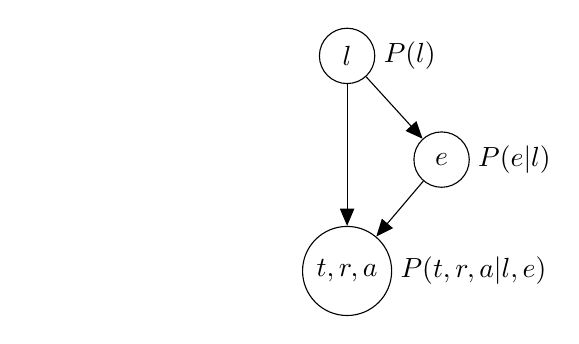
\begin{tikzpicture}[scale=0.33]
  \node[latent] (l) {$l$};
  \node[latent, below=of l, xshift=1.2cm, yshift=0.4cm] (e) {$e$};
  \node[latent, below=of l, yshift=-0.8cm] (tra) {$\ t,r,a\ $};
  \edge {l} {e};
  \edge {l,e} {tra};

  \node[const, right=of l] (pl) {$P(l)$};
  \node[const, right=of e] (pe) {$P(e|l)$};
  \node[const, right=of tra] (ptra) {$P(t,r,a|l,e)$};

  \node[invisible, xshift=-4cm] (inv) {};
\end{tikzpicture}
\end{textblock}
}


\only<8-10>{
\begin{textblock}{160}(40,38)
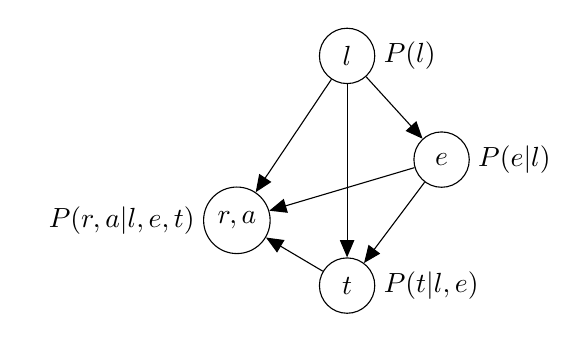
\begin{tikzpicture}[scale=0.33]
  \node[latent] (l) {$l$};
  \node[latent, below=of l, xshift=1.2cm, yshift=0.4cm] (e) {$e$};
  \node[latent, below=of l, yshift=-1.2cm] (t) {$t$};
  \node[latent, below=of l, yshift=-0.3cm, xshift=-1.4cm] (ra) {$\ r, a\ $};

  \edge {l} {e};
  \edge {l,e} {t};
  \edge {l,e,t} {ra};

  \node[const, right=of l] (pl) {$P(l)$};
  \node[const, right=of e] (pe) {$P(e|l)$};
  \node[const, right=of t] (pt) {$P(t|l,e)$};
  \node[const, left=of ra] (pra) {$P(r,a|l,e,t)$};
  \node[invisible, xshift=-4cm] (inv) {};
\end{tikzpicture}
\end{textblock}
}


\only<11>{
\begin{textblock}{160}(40,38)
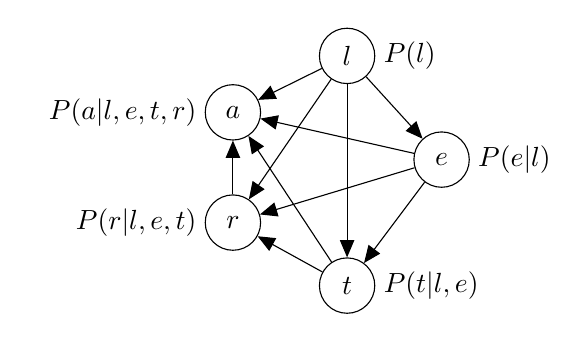
\begin{tikzpicture}[scale=0.33]
  \node[latent] (l) {$l$};
  \node[latent, below=of l, xshift=1.2cm, yshift=0.4cm] (e) {$e$};
  \node[latent, below=of l, yshift=-1.2cm] (t) {$t$};
  \node[latent, below=of l, yshift=-0.4cm, xshift=-1.45cm] (r) {$r$};
  \node[latent, below=of l, yshift=1cm, xshift=-1.45cm] (a) {$a$};


  \edge {l} {e};
  \edge {l,e} {t};
  \edge {l,e,t} {r};
  \edge {l,e,t,r} {a};

  \node[const, right=of l] (pl) {$P(l)$};
  \node[const, right=of e] (pe) {$P(e|l)$};
  \node[const, right=of t] (pt) {$P(t|l,e)$};
  \node[const, left=of r] (pr) {$P(r|l,e,t)$};
  \node[const, left=of a] (pa) {$P(a|l,e,t,r)$};
  \node[invisible, xshift=-4cm] (inv) {};
\end{tikzpicture}
\end{textblock}
}

\only<12>{
\begin{textblock}{160}(40,38)
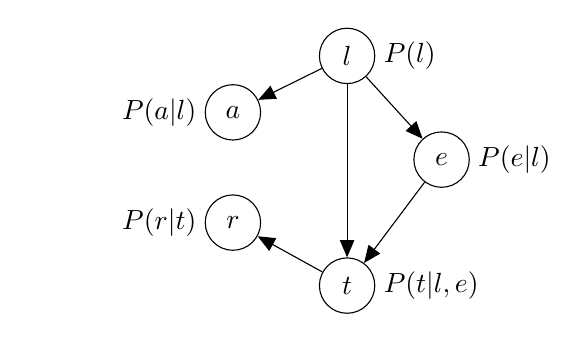
\begin{tikzpicture}[scale=0.33]
  \node[latent] (l) {$l$};
  \node[latent, below=of l, xshift=1.2cm, yshift=0.4cm] (e) {$e$};
  \node[latent, below=of l, yshift=-1.2cm] (t) {$t$};
  \node[latent, below=of l, yshift=-0.4cm, xshift=-1.45cm] (r) {$r$};
  \node[latent, below=of l, yshift=1cm, xshift=-1.45cm] (a) {$a$};


  \edge {l} {e};
  \edge {l,e} {t};
  \edge {t} {r};
  \edge {l} {a};

  \node[const, right=of l] (pl) {$P(l)$};
  \node[const, right=of e] (pe) {$P(e|l)$};
  \node[const, right=of t] (pt) {$P(t|l,e)$};
  \node[const, left=of r] (pr) {$P(r|t)$};
  \node[const, left=of a] (pa) {$P(a|l)$};
  \node[invisible, xshift=-4cm] (inv) {};
\end{tikzpicture}
\end{textblock}
}

\only<13->{
\begin{textblock}{160}(0,38) \Large \centering
Hay $5! = 120$ posibles descomposiciones \\[0.3cm]

\only<14>{¿Cuál de todas ellas usar?}
\end{textblock}
}
\end{frame}
%
% \begin{frame}[plain]
% %
% % \begin{textblock}{160}(0,-50)
% % \includegraphics[width=1\textwidth,page=1]{../../../auxiliar/download/argumentos2.jpg}
% % \end{textblock}
%
% \begin{textblock}{160}(0,-60)
% \includegraphics[width=1\textwidth,page=1]{../../../auxiliar/download/argumentos3.png}
% \end{textblock}
%
% \end{frame}


\begin{frame}[plain]
\begin{textblock}{160}(0,3)
 \centering \LARGE  Redes bayesianas \\ \large
 \only<1-8>{Historias causales}\only<9>{Sistemas complejos}
 \end{textblock}


\only<1-6>{
\begin{textblock}{140}(10,18)
La \textbf{alarma} ($a$) de una casa se activa cuando alguien \textbf{entra} ($e$) sin apagarla. Si la alarma se activa, la dueña recibe una \textbf{llamada} ($l$) de la central de seguridad. La alarma se puede activar por otros motivos, como los \textbf{terremotos} ($t$) que no son infrecuentes en la ciudad. Siempre que se produce un terremoto, en las \textbf{redes} ($r$) se habla casi exclusivamente de eso.
 \end{textblock}
}

\only<2-5>{
\begin{textblock}{160}(10,46)
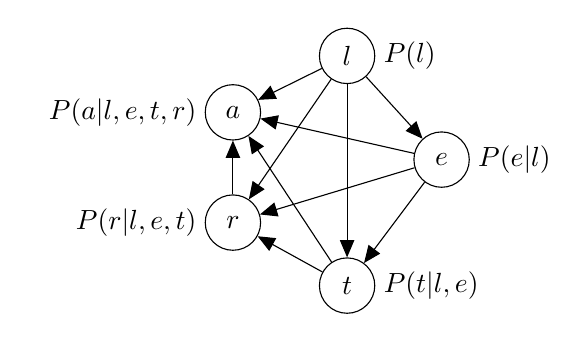
\begin{tikzpicture}[scale=0.33]
  \node[latent] (l) {$l$};
  \node[latent, below=of l, xshift=1.2cm, yshift=0.4cm] (e) {$e$};
  \node[latent, below=of l, yshift=-1.2cm] (t) {$t$};
  \node[latent, below=of l, yshift=-0.4cm, xshift=-1.45cm] (r) {$r$};
  \node[latent, below=of l, yshift=1cm, xshift=-1.45cm] (a) {$a$};


  \edge {l} {e};
  \edge {l,e} {t};
  \edge {l,e,t} {r};
  \edge {l,e,t,r} {a};

  \node[const, right=of l] (pl) {$P(l)$};
  \node[const, right=of e] (pe) {$P(e|l)$};
  \node[const, right=of t] (pt) {$P(t|l,e)$};
  \node[const, left=of r] (pr) {$P(r|l,e,t)$};
  \node[const, left=of a] (pa) {$P(a|l,e,t,r)$};
  \node[invisible, xshift=-4cm] (inv) {};
\end{tikzpicture}
\end{textblock}
}

\only<3-6>{
\begin{textblock}{70}(80,50) \centering \Large
¿Cómo podemos definir

la probabilidad conjunta? \\[0.3cm] \large


\only<4>{
 $$P(t|l,e) = \ ?$$
}
\only<5-6>{
 $$P(t)\,P(e)\,P(a|e,t)\,P(l|a)P(r|t)$$
}
\end{textblock}
}



\only<6>{
\begin{textblock}{160}(10,46)
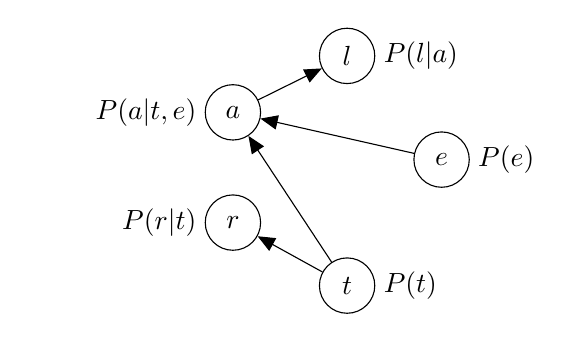
\begin{tikzpicture}[scale=0.33]
  \node[latent] (l) {$l$};
  \node[latent, below=of l, xshift=1.2cm, yshift=0.4cm] (e) {$e$};
  \node[latent, below=of l, yshift=-1.2cm] (t) {$t$};
  \node[latent, below=of l, yshift=-0.4cm, xshift=-1.45cm] (r) {$r$};
  \node[latent, below=of l, yshift=1cm, xshift=-1.45cm] (a) {$a$};


  \edge {a} {l};
  \edge {t,e} {a};
  \edge {t} {r};

  \node[const, right=of l] (pl) {$P(l|a)$};
  \node[const, right=of e] (pe) {$P(e)$};
  \node[const, right=of t] (pt) {$P(t)$};
  \node[const, left=of r] (pr) {$P(r|t)$};
  \node[const, left=of a] (pa) {$P(a|t,e)$};
  \node[invisible, xshift=-4cm] (inv) {};
\end{tikzpicture}
\end{textblock}
}

\only<7->{
\begin{textblock}{80}(05,16) \centering
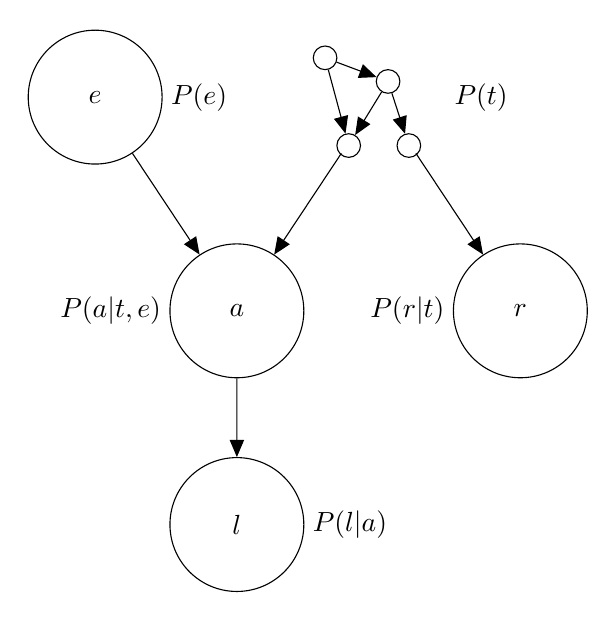
\begin{tikzpicture}[scale=0.33]
  \node[latent, minimum size=1.7cm] (e) {$e$};

  \node[latent, minimum size=1.7cm, below=of e, xshift=1.8cm] (a) {$a$};

  \node[latent,minimum size=1.7cm, above=of a, xshift=1.8cm] (t) {$t$};
  \node[latent,minimum size=1.7cm, below=of t, xshift=1.8cm] (r) {$r$};

  \node[latent, minimum size=1.7cm,below=of a] (l) {$l$};

  \onslide<9->{
  \node[latent,minimum size=1.75cm, draw=white, fill=white, above=of a, yshift=-0.025cm, xshift=1.8cm] (t2) {};

  \node[latent,minimum size=0.3cm, above=of a, yshift=0.085cm, xshift=1.42cm] (sub_t1) {};
  \node[latent,minimum size=0.3cm, right=of sub_t1, xshift=-0.55cm] (sub_t2) {};

  \node[latent,minimum size=0.3cm, above=of sub_t1, yshift=-0.5cm, xshift=0.5cm] (sub_t3) {};
  \node[latent,minimum size=0.3cm, above=of sub_t1, yshift=-0.2cm, xshift=-0.3cm] (sub_t4) {};

  }

  \edge {a} {l};
  \edge {t,e} {a};
  \edge {t} {r};
  \onslide<9->{
    \edge {sub_t4, sub_t3} {sub_t1};
    \edge {sub_t3} {sub_t2};
    \edge {sub_t4} {sub_t3};
  }
  \node[const, right=of l] (pl) {$P(l|a)$};
  \node[const, right=of e] (pe) {$P(e)$};
  \only<7-8>{\node[const, right=of t] (pt) {$P(t)$};}
  \node[const, left=of r] (pr) {$P(r|t)$};
  \node[const, left=of a] (pa) {$P(a|t,e)$};
  %\node[invisible, yshift=-1cm] (inv) {};
\end{tikzpicture}
\end{textblock}
}

\only<8->{
\begin{textblock}{75}(80,36) \centering \Large
Cada variable resumen el compor-

tamiento de un sistema complejo
\end{textblock}
}

\end{frame}


\begin{frame}[plain]
\begin{textblock}{160}(0,3)
 \centering \LARGE Redes bayesianas \\ \large
\only<1-13>{Sistemas complejos}\only<14->{Historias causales}
 \end{textblock}

\only<1-5>{
\begin{textblock}{160}(0,18) \centering
\only<1>{\includegraphics[ trim=0.6cm 0cm 0.6cm 0cm, clip, width=0.7\textwidth,page=1]{../../../auxiliar/download/terremoto/terremoto_modelo_1.jpg}}%
\only<2>{\includegraphics[trim=0.6cm 0cm 0.6cm 0cm, clip, width=0.7\textwidth,page=1]{../../../auxiliar/download/terremoto/terremoto_modelo_2.jpg}}%
\only<3>{\includegraphics[trim=0.6cm 0cm 0.6cm 0cm, clip,width=0.7\textwidth,page=1]{../../../auxiliar/download/terremoto/terremoto_modelo_3.jpg}}%
\only<4>{\includegraphics[trim=0.6cm 0cm 0.6cm 0cm, clip,width=0.7\textwidth,page=1]{../../../auxiliar/download/terremoto/terremoto_modelo_4.jpg}}%
\only<5>{\includegraphics[trim=0.6cm 0cm 0.6cm 0cm, clip,width=0.7\textwidth,page=1]{../../../auxiliar/download/terremoto/terremoto_modelo_5.jpg}}
 \end{textblock}
}

\only<6-12>{
\begin{textblock}{160}(0,18) \centering
\only<6>{\includegraphics[width=0.7\textwidth,page=1]{../../../auxiliar/download/terremoto/japonsito2.jpg}}%
\only<7>{\includegraphics[width=0.7\textwidth,page=1]{../../../auxiliar/download/terremoto/japonsito3.jpg}}%
\only<8>{\includegraphics[width=0.7\textwidth,page=1]{../../../auxiliar/download/terremoto/japonsito5.jpg}}%
\only<9>{\includegraphics[width=0.7\textwidth,page=1]{../../../auxiliar/download/terremoto/japonsito7.jpg}}%
\only<10>{\includegraphics[width=0.7\textwidth,page=1]{../../../auxiliar/download/terremoto/japonsito11.jpg}}%
\only<11>{\includegraphics[width=0.7\textwidth,page=1]{../../../auxiliar/download/terremoto/japonsito14.jpg}}%
\only<12>{\includegraphics[width=0.7\textwidth,page=1]{../../../auxiliar/download/terremoto/japonsito20.jpg}}%
\end{textblock}
}

\only<13->{
\begin{textblock}{80}(02,14)
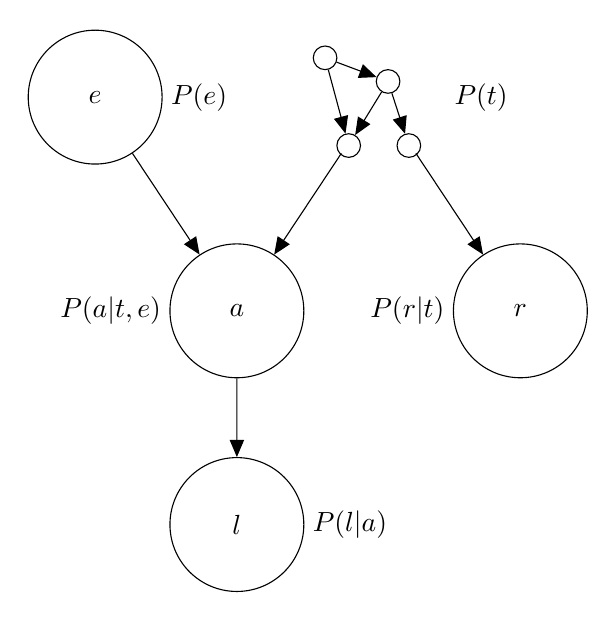
\begin{tikzpicture}[scale=0.33]
  \node[latent, minimum size=1.7cm] (e) {$e$};

  \node[latent, minimum size=1.7cm, below=of e, xshift=1.8cm] (a) {$a$};

  \node[latent,minimum size=1.7cm, above=of a, xshift=1.8cm] (t) {$t$};
  \node[latent,minimum size=1.7cm, below=of t, xshift=1.8cm] (r) {$r$};

  \node[latent, minimum size=1.7cm,below=of a] (l) {$l$};

  \onslide<13>{
  \node[latent,minimum size=1.75cm, draw=white, fill=white, above=of a, yshift=-0.025cm, xshift=1.8cm] (t2) {};

  \node[latent,minimum size=0.3cm, above=of a, yshift=0.085cm, xshift=1.42cm] (sub_t1) {};
  \node[latent,minimum size=0.3cm, right=of sub_t1, xshift=-0.55cm] (sub_t2) {};

  \node[latent,minimum size=0.3cm, above=of sub_t1, yshift=-0.5cm, xshift=0.5cm] (sub_t3) {};
  \node[latent,minimum size=0.3cm, above=of sub_t1, yshift=-0.2cm, xshift=-0.3cm] (sub_t4) {};

  }

  \edge {a} {l};
  \edge {t,e} {a};
  \edge {t} {r};
  \onslide<13>{
    \edge {sub_t4, sub_t3} {sub_t1};
    \edge {sub_t3} {sub_t2};
    \edge {sub_t4} {sub_t3};
  }
  \node[const, right=of l] (pl) {$P(l|a)$};
  \node[const, right=of e] (pe) {$P(e)$};
  \only<14->{\node[const, right=of t] (pt) {$P(t)$};}
  \node[const, left=of r] (pr) {$P(r|t)$};
  \node[const, left=of a] (pa) {$P(a|t,e)$};
  %\node[invisible, yshift=-1cm] (inv) {};
\end{tikzpicture}
\end{textblock}
}


\only<15->{
\begin{textblock}{85}(75,34)
  \begin{itemize}
   \only<15->{\item[$\bullet$] Define la probabilidad conjunta}
   \only<16->{\item[$\bullet$] {Expresa las hipótesis de forma intuitiva}}
   \only<17->{\item[$\bullet$] {Permite hacer inferencia eficientemente}}
  \end{itemize}
\end{textblock}
}


\end{frame}


%\begin{frame}[plain]
% \begin{textblock}{160}(0,3)
%  \centering \Large
%  Modelo Causal
%  \end{textblock}
%  \centering
%  \vspace{0.75cm}
%
%  \tikz{
%     \node[det] (l) {$l$} ; %
%     \node[det, above=of l] (a) {$a$} ; %
%     \node[det, above=of a,xshift=1.5cm] (t) {$t$} ; %
%     \node[det, above=of a,xshift=-1.5cm] (e) {$e$} ; %
%     \node[det, below=of t,xshift=1.5cm] (r) {$r$} ; %
%
%     \edge {a} {l};
%     \edge {t,e} {a};
%     \edge {t} {r};
%
%     \node[const, left= of e, xshift=-0.1cm] (cpd_e) {Entradera:};
%     \node[const, right= of t, xshift=0.1cm] (cpd_t) {:Terremoto};
%     \node[const, left= of a, xshift=-0.1cm] (cpd_a) {Alarma:};
%     \node[const, right= of r, xshift=0.1cm] (cpd_r) {:Redes};
%     \node[const, left= of l, xshift=-0.1cm] (cpd_l) {Llamada:};
%
%     }
%
%
%
%  \end{frame}

\begin{frame}[plain]
\begin{textblock}{160}(0,3) \centering \LARGE Método de especificación \\ \large
  Grafo de factorización (factor graph)
\end{textblock}

\begin{textblock}{40}(1,9)
\centering
\begin{figure}[H]
\centering
  \scalebox{0.9}{
\tikz{ %


        \node[factor] (fa) {} ;
        \node[const,right=of fa] (pa) {$P(a|e,t)$} ;
        \node[latent, minimum size = 0.9cm,below=of fa, yshift=0.1cm] (a) {\text{\Large $a$}} ; %

        \node[factor, below=of a] (fl) {} ;
        \node[const,right=of fl] (pl) {$P(l|a)$} ;
        \node[latent, minimum size = 0.9cm, below=of fl,yshift=0.1cm] (l) {\text{\Large$l$}} ; %

        \node[latent, minimum size = 0.9cm, above=of fa, xshift=-1.6cm,yshift=-0.1cm] (e) {\text{\Large$e$}} ; %
        \node[factor, above=of e,yshift=-0.1cm] (fe) {} ;
        \node[const,right=of fe] (pe) {$P(e)$} ;

        \node[latent, minimum size = 0.9cm, above=of fa, xshift=1.6cm,yshift=-0.1cm] (t) {\text{\Large$t$}} ; %
        \node[factor, above=of t,yshift=-0.1cm] (ft) {} ;
        \node[const,right=of ft] (pt) {$P(t)$} ;
        \node[factor, below=of t, xshift=1.6cm,yshift=0.1cm] (fr) {} ;
        \node[latent,minimum size = 0.9cm, below=of fr,yshift=0.1cm] (r) {\text{\Large$r$}} ; %
        \node[const,right=of fr] (pr) {$P(r|t)$} ;

        \edge[-] {fa} {e,t};
        \edge[-] {fr} {t};
        \edge[-] {fl} {a};

        \only<2>{
          \edge {fl} {l};
          \edge {fr} {r};
          \edge {fa} {a};
          \edge {fe} {e};
          \edge {ft} {t};
        }
        \only<1>{
          \edge[-] {fl} {l};
          \edge[-] {fr} {r};
          \edge[-] {fa} {a};
          \edge[-] {fe} {e};
          \edge[-] {ft} {t};
        }

        }
}
\end{figure}
\end{textblock}

\begin{textblock}{115}(45,30)

 \centering Nodos: \\ variables y funciones

 \vspace{1cm}

 \centering Ejes: \\
  ``la variable $v$ es argumento de la funci\'on $P$''

\end{textblock}
\end{frame}


% \begin{frame}[plain]
% \begin{textblock}{160}(0,3)
%  \centering \Large El truco de la factorización
% \end{textblock}
% \vspace{1.5cm} \centering
%
% \begin{equation*}
% \sum \prod = \prod \sum
% \end{equation*}
%
% $a_1 \, b_1 + a_1 \, b_2 + a_2 \, b_1 + a_2 \, b_2  = (a1 + a_2) \, (b_1 + b_2)$
%
% \pause
%
% \begin{equation*}
%    P(a^1) = \Big(\sum_l P(l|a^1) \Big) \Big(\sum_{e,t} P(e)P(t)P(a^1|t,e)(\sum_r P(r|t)) \Big)
% \end{equation*}
%
%   \includegraphics[width=0.35\textwidth]{../../../auxiliar/download/sum_product.png}
%
% \end{frame}
%



\begin{frame}[plain,noframenumbering]
\begin{textblock}{160}(0,43)
\includegraphics[width=1\textwidth]{../../../auxiliar/download/modelosGraficos}
\end{textblock}


\begin{textblock}{160}(4,4)
\LARGE \textcolor{black!85}{\fontsize{22}{0}\selectfont \textbf{Especificación y evaluación de modelos}} \\
\LARGE Parte 2
\end{textblock}
% \begin{textblock}{160}(4,12)
% \LARGE \textcolor{black!85}{\fontsize{22}{0}\selectfont \textbf{algoritmos de inferencia}}
% \end{textblock}

\begin{textblock}{150}(5,29)

Especificación de estructuras causales dinámicas. Identificación de modelo causal. El problema histórico de la aplicación estricta de las reglas de la probabilidad. Regresión lineal. Overfitting y el balance natural de las reglas de la probabilidad.
\end{textblock}
%
% \begin{textblock}{55}[0,0](72,23)
% \begin{turn}{0}
% \parbox{10cm}{\sloppy\setlength\parfillskip{0pt}
% \textcolor{black!85}{Unidad 1} \\
% \small\textcolor{black!85}{Aprendizaje basado en modelos. Distribuciones de creencias} \\
% \small\textcolor{black!85}{honestas. Las reglas de razonamiento en contextos de} \\
% \small\textcolor{black!85}{incertidumbre. Métodos gráficos de especificación matemática} \\
% \small\textcolor{black!85}{de argumentos causales. Evaluación de modelos causales alternativos} \\
% }
% \end{turn}
% \end{textblock}

\end{frame}

%
\begin{frame}[plain]
\begin{textblock}{160}(0,3)
\centering \LARGE Capítulo 19 - Evaluating Causal models \large \\
Causal Inference for the Brave and the True
\end{textblock}

\begin{quotation}
It isn't obvious at all how we achieve anything like a train-test paradigm in the case of causal inference. That's because causal inference is interested in estimating an unobservable variable.
\end{quotation}

\end{frame}


\begin{frame}[plain]
\begin{textblock}{160}(0,3) \centering
 \LARGE Flujo de inferencia \\
 \large por descomposición de las reglas de la probabilidad
\end{textblock}

\only<2->{
\begin{textblock}{80}(45,30)
\begin{description}
 \onslide<3->{\item[$v(n)$ :] Vecinos del nodo $n$}
 \item[$m_{x \rightarrow f}(x)$ :] Mensaje de variable $x$ a factor $f$
 \item[$m_{f \rightarrow x}(x)$ :] Mensaje de factor $f$ a variable $x$
\end{description}
\end{textblock}
}


\only<2-3>{
\begin{textblock}{100}(40,19)
\centering
Pasaje de mensajes entre los nodos de la red causal
\end{textblock}
}


\only<4->{
\begin{textblock}{80}(45,17)
\begin{equation*}
P(x) = \prod_{f \in v(x)} m_{f \rightarrow x}(x)
\end{equation*}
\end{textblock}
}
%
% \only<5-10>{
% \begin{textblock}{80}(45,56)
% \begin{equation*}\label{eq:m_v_f}
% m_{x \rightarrow f}(x) = \prod_{h \in \only<6>{\textcolor{red}}{v(x) \setminus \{f\}} } m_{h \rightarrow x}(x)
% \end{equation*}
% \end{textblock}
% }
%
% \only<7-10>{
% \begin{textblock}{80}(45,68)
% \begin{equation*}\label{eq:m_f_v}
%  m_{f \rightarrow x}(x) = \onslide<9->{\sum_{\bm{h}} \Big(} \onslide<8->{f(\bm{h},x)} \prod_{h \in v(f) \setminus \{x\} } m_{h \rightarrow f}(h) \onslide<9->{\Big)}
% \end{equation*}
% \end{textblock}
% }

\only<1->{
\begin{textblock}{40}(0,20)
\centering
\begin{figure}[H]
\centering
  \scalebox{.8}{
\tikz{ %


        \node[factor] (fa) {} ;
        \node[latent, below=of fa, minimum size=0.55cm, yshift=0.4cm] (a) {$a$} ; %

        \node[factor, below=of a, yshift=0.4cm] (fl) {} ;
        \node[latent, below=of fl, minimum size=0.55cm,yshift=0.4cm] (l) {$l$} ; %

        \node[latent, above=of fa, minimum size=0.55cm, xshift=-0.8cm, yshift=-0.4cm] (e) {$e$} ; %
        \node[factor, above=of e, yshift=-0.4cm] (fe) {} ;

        \node[latent,minimum size=0.55cm, above=of fa, xshift=0.8cm, yshift=-0.4cm] (t) {$t$} ; %
        \node[factor, above=of t, yshift=-0.4cm] (ft) {} ;
        \node[factor, below=of t, xshift=0.8cm, yshift=0.4cm] (fr) {} ;
        \node[latent,minimum size=0.55cm, below=of fr, yshift=0.4cm] (r) {$r$} ; %

        \edge[-] {fa} {e,t};
        \edge {fa} {a};
        \edge {fe} {e};
        \edge {ft} {t};
        \edge[-] {fr} {t};
        \edge {fr} {r};
        \edge[-] {fl} {a};
        \edge {fl} {l};
        }
}
\end{figure}
\end{textblock}
}

\only<4->{
\begin{textblock}{160}(0,87)
\centering \tiny
\href{https://ieeexplore.ieee.org/stamp/stamp.jsp?arnumber=910572}{Kschischang FR, Frey BJ, Loeliger HA. Factor graphs and the sum-product algorithm. 2001}
\end{textblock}
}

\end{frame}


\begin{frame}[plain]
\begin{textblock}{160}(0,3)
\centering \LARGE Evaluación de modelos causales
\end{textblock}

\only<1->{

\begin{textblock}{140}(10,12)
\centering
\includegraphics[width=0.66\textwidth]{../../../figuras/MontyHall/monty_hall_selection.pdf} \hspace{2cm}
\end{textblock}

\begin{textblock}{80}(86,12)
\centering
\scalebox{0.5}{
\tikz{

    \node[latent] (d) {\includegraphics[width=0.10\textwidth]{../../../auxiliar/download/dedo.png}} ;
    \node[const,left=of d] (nd) {\Large $s$} ;

    \node[latent, above=of d, xshift=-1.5cm] (r) {\includegraphics[width=0.12\textwidth]{../../../auxiliar/download/regalo.png}} ;
    \node[const,left=of r] (nr) {\Large $r$} ;


    \node[latent, fill=black!30, above=of d, xshift=1.5cm] (c) {\includegraphics[width=0.12\textwidth]{../../../auxiliar/download/cerradura.png}} ;
    \node[const,left=of c] (nc) {\Large $c$} ;

    \edge {r,c} {d};
}
}
\end{textblock}


\begin{textblock}{80}(86,48)
\centering
\scalebox{0.5}{
 \tikz{
    \node[latent,] (r) {\includegraphics[width=0.12\textwidth]{../../../auxiliar/download/regalo.png}} ;
    \node[const,left=of r] (nr) {\Large $r$} ;


    \node[latent, below=of r] (d) {\includegraphics[width=0.10\textwidth]{../../../auxiliar/download/dedo.png}} ;
    \node[const, left=of d] (nd) {\Large $s$} ;

    \edge {r} {d};

}
}
\end{textblock}
}


\only<2>{
\begin{textblock}{140}(10,76) \centering
  \Large ¿Qué pasaría con la evaluación de modelos si la persona que da la pista a veces se olvida de tener en cuenta la caja que elegimos?
\end{textblock}
}


\end{frame}


\begin{frame}[plain]
\begin{textblock}{160}(0,3) \centering \LARGE Mecanismos causales dinámicos \\ \large
\end{textblock}

\only<1-2>{
\begin{textblock}{160}(0,14)
\centering
\scalebox{0.6}{
\tikz{
    \node[invisible] (id) {};
    \node[latent, left=of id, xshift=-3.5cm] (d) {\includegraphics[width=0.05\textwidth]{../../../auxiliar/download/dedo.png}} ;
    \node[const,left=of d] (nd) {\Large $P(s_t|r_t)$} ;
    \node[const, below=of d, yshift=-0.2cm] (restricciones) {$s_t \neq r_t$};


    \node[latent, above=of d, xshift=-1.5cm] (r) {\includegraphics[width=0.06\textwidth]{../../../auxiliar/download/regalo.png}} ;
    \node[const,left=of r] (nr) {\Large $P(r_t)$} ;


    \node[latent, fill=black!30, above=of d, xshift=1.5cm] (c) {\includegraphics[width=0.06\textwidth]{../../../auxiliar/download/cerradura.png}} ;
    \node[const,left=of c] (nc) {\Large $P(c_t)$} ;

    \node[invisible, above=of c, yshift=0.1cm] (ic) {};


    \edge {r} {d};
    %\plate {repeticiones} {(nr)(c)(restricciones)} {$t \in \{0, \dots, T-1\}$};


    \node[invisible] (id_1) {};
    \node[latent, left=of id, xshift=3.5cm] (d_1) {\includegraphics[width=0.05\textwidth]{../../../auxiliar/download/dedo.png}} ;
    \node[const,left=of d_1] (nd) {\Large $P(s_t|r_t,c_t)$} ;
    \node[const, below=of d_1, yshift=-0.2cm] (restricciones_1) {$s_t \neq r_t \text{, } s_t \neq c_t$};


    \node[latent, above=of d_1, xshift=-1.5cm] (r_1) {\includegraphics[width=0.06\textwidth]{../../../auxiliar/download/regalo.png}} ;
    \node[const,left=of r_1] (nr_1) {\Large $P(r_t)$} ;


    \node[latent, fill=black!30, above=of d_1, xshift=1.5cm] (c_1) {\includegraphics[width=0.06\textwidth]{../../../auxiliar/download/cerradura.png}} ;
    \node[const,left=of c_1] (nc_1) {\Large $P(c_t)$} ;

    \edge {r_1,c_1} {d_1};

    \node[latent, yshift=4.8cm, xshift=-2.4cm ] (a) {\includegraphics[width=0.06\textwidth]{../../../auxiliar/static/prendido-apagado.png}};
    \node[const,left=of a] (pm) {\Large $P(a_t|p) $} ;
    \node[const,right=of a] (nm) {\Large Acción} ;


    \node[latent, above=of a, yshift=-0.3cm] (m) {\includegraphics[width=0.06\textwidth]{../../../auxiliar/static/cerebro.jpg}};
    \node[const,left=of m] (pm) {\Large $P(p) $} ;
    \node[const,right=of m] (nm) {\Large Probabilidad acción} ;

    \vgate {M} {(nr)(ic)(restricciones)} {$\bm{a_t=0}$} {(nr_1)(c_1)(restricciones_1)} {$\bm{a_t=1}$} {a};


    \edge {m} {a};

    \plate {B} {(a)(M)} {$t \in \{0, \dots, T-1\} $};
}
}
\end{textblock}
}

\only<2>{
\begin{textblock}{160}(0,78) \centering \Large
Veamos la especificación precisa usando factor graphs.
\end{textblock}
}

\only<3-5>{
\begin{textblock}{157}(0,14) \centering
\scalebox{0.6}{
\tikz{
    \node[latent] (d) {\includegraphics[width=0.05\textwidth]{../../../auxiliar/download/dedo.png}} ;
    \node[factor, above=of d] (fd) {};
    \node[const, right=of fd, yshift=-0.1cm] (nd) {\text{\Large $P(s_t|r_t, c_t, a_t)$}};
    \node[latent, above=of fd, xshift=-2.5cm, yshift=-0.2cm] (r) {\includegraphics[width=0.06\textwidth]{../../../auxiliar/download/regalo.png}} ;
    \node[factor, above=of r] (fr) {};
    \node[const, left=of fr] (nr) {\text{\Large $P(r_t)$}};

    \node[latent, fill=black!30, above=of fd, xshift=2.5cm, yshift=-0.2cm] (c) {\includegraphics[width=0.06\textwidth]{../../../auxiliar/download/cerradura.png}} ;
    \node[factor, above=of c] (fc) {};
    \node[const, right=of fc] (nc) {\text{\Large $P(c_t)$}};

    \node[latent, yshift=4.8cm] (a) {\includegraphics[width=0.06\textwidth]{../../../auxiliar/static/prendido-apagado.png}};
    \node[factor, above=of a] (fa) {};
    \node[const, right=of fa] (na) {\text{\Large $P(a_t|p)$}};
    \node[latent, above=of fa, yshift=-0.3cm] (m) {\includegraphics[width=0.06\textwidth]{../../../auxiliar/static/cerebro.jpg}};
    \node[factor, above=of m] (fm) {};
    \node[const, right=of fm] (nm) {\text{\Large $P(p)$}};


    \edge[-] {a,r,c} {fd};
    \edge {fd} {d};
    \edge {fc} {c};
    \edge {fr} {r};
    \edge {fm} {m};
    \edge {m} {a};

    \plate {B} {(a)(r)(c)(d)(fa)(na)(nc)(nr)} {$t \in \{0, \dots, T-1\} $};
}
}
\end{textblock}
}

\only<4-5>{
\begin{textblock}{55}(0,54)
$$P(s_t|r_t, c_t, a_t=0) = P(s_t|r_t)$$
\end{textblock}
}

\only<5>{
\begin{textblock}{50}(104,54)
$$P(s_t|r_t, c_t, a_t=1) = P(s_t|r_t,c_t)$$
\end{textblock}
}

\only<6-7>{
\begin{textblock}{140}(10,34)
\ \ \ \ $\bullet$ Minka, T; Winn, J. \textit{Gates}; Advances in Neural Information Processing Systems. 2008. \href{https://proceedings.neurips.cc/paper_files/paper/2008/file/4b0a59ddf11c58e7446c9df0da541a84-Paper.pdf}{(Descargar)}. \\[0.3cm]

\ \ \ \ $\bullet$ Winn, J. \textbf{Causality with Gates}; Proceedings of Machine Learning Research. 2012. \href{http://proceedings.mlr.press/v22/winn12/winn12.pdf}{(Descargar)}. \\[0.3cm]

\centering

\only<7>{
\begin{quotation}
La notación de compuertas (gates) permite especificar mecanismos causales dinámicos que dependen del contexto.
\end{quotation}
}
\end{textblock}
}

\end{frame}

\begin{frame}[plain]
\begin{textblock}{160}(0,2) \centering \LARGE Mecanismos causales dinámicos \\ \large
\only<1-5>{Gates}\only<6>{Evaluación de modelos}
\end{textblock}

\only<1-4>{
\begin{textblock}{160}(0,15) \centering
\scalebox{0.6}{
\tikz{
    \node[latent] (d) {\includegraphics[width=0.05\textwidth]{../../../auxiliar/download/dedo.png}} ;
    \node[invisible, below=of d, yshift=0.6cm] (inv_d) {} ;
    \node[factor, above=of d, xshift=-0.4cm] (fd0) {};
    \node[invisible, above=of fd0, xshift=-0.4cm, yshift=0.2cm] (inv_fd0) {};
    \only<1,3->{\node[factor, above=of d, xshift=0.4cm] (fd1) {};}
    \only<2>{\node[factor, fill=black!10, draw=black!10, above=of d, xshift=0.4cm] (fd1) {};}
    \node[invisible, above=of fd1, xshift=0.4cm, yshift=0.2cm] (inv_fd1) {};

    \vgate {fd} {(fd0)(inv_fd0)} {\only<1-2,4>{$0$}\only<3>{\textcolor{black!15}{$0$}}} {(fd1)(inv_fd1)} {\only<1,3->{$1$}\only<2>{\textcolor{black!15}{$1$}}} {a};

    \node[const, left=of fd] (nfd0) {\only<1-2,4>{\textcolor{black}{\Large $P(s_t|r_t)$}}\only<3>{\textcolor{black!15}{\Large $P(s_t|r_t)$}}};
    \node[const, right=of fd] (nfd1) {\only<1,3->{\textcolor{black}{\Large $P(s_t|r_t,c_t)$}}\only<2>{\textcolor{black!15}{\Large $P(s_t|r_t,c_t)$}}};


    \node[latent, above=of fd, xshift=-2.5cm, yshift=-0.2cm] (r) {\includegraphics[width=0.06\textwidth]{../../../auxiliar/download/regalo.png}} ;
    \node[factor, above=of r] (fr) {};
    \node[const, left=of fr] (nr) {\text{\Large $P(r_t)$}};

    \node[latent, fill=black!30, above=of fd, xshift=2.5cm, yshift=-0.2cm] (c) {\includegraphics[width=0.06\textwidth]{../../../auxiliar/download/cerradura.png}} ;
    \node[factor, above=of c] (fc) {};
    \node[const, right=of fc] (nc) {\text{\Large $P(c_t)$}};

    \node[latent, line width=0cm, yshift=4.8cm] (a) {\includegraphics[width=0.06\textwidth]{../../../auxiliar/static/prendido-apagado.png}};
    \only<2-3>{\node[latent, line width=0.1cm, yshift=4.8cm] (a1) {\includegraphics[width=0.06\textwidth]{../../../auxiliar/static/prendido-apagado.png}};}
    \node[factor, above=of a] (fa) {};
    \only<1,4>{\node[const, right=of fa] (na) {\text{\Large $P(a_t|p)$}};}
    \only<2>{\node[const, right=of fa] (na) {\text{\Large $P(a_t=0|p)$}};}
    \only<3>{\node[const, right=of fa] (na) {\text{\Large $P(a_t=1|p)$}};}


    \node[latent, above=of fa, yshift=-0.3cm] (m) {\includegraphics[width=0.06\textwidth]{../../../auxiliar/static/cerebro.jpg}};
    \node[factor, above=of m] (fm) {};
    \node[const, right=of fm] (nm) {\text{\Large $P(p)$}};


    \only<1,3->{\edge[-] {r,c} {fd1};}
    \only<2>{\edge[draw=black!15,-] {r,c} {fd1};}

    \only<1-2,4>{\edge[-] {r} {fd0};}
    \only<3>{\edge[draw=black!15,-] {r} {fd0};}
    \only<1,3->{\edge {fd1} {d};}
    \only<2>{\edge[draw=black!15] {fd1} {d};}

    \only<1-2,4>{\edge {fd0} {d};}
    \only<3>{\edge[draw=black!15] {fd0} {d};}
    \edge {fc} {c};
    \edge {fr} {r};
    \edge {fm} {m};
    \edge {m} {a};

    \plate {B} {(inv_d)(a)(r)(c)(fa)(na)(nc)(nr)} {$t \in \{0, \dots, T-1\} $};
}
}
\end{textblock}
}

\only<4>{
\begin{textblock}{160}(0,85) \centering
\text{\footnotesize $P(s_t|r_t, c_t, a_t) = P(s_t|r_t)^{\mathbb{I}(a_t=0)} P(s_t|r_t,c_t)^{\mathbb{I}(a_t=1)} $}
\end{textblock}
}

\only<5>{
\begin{textblock}{160}(0,15) \centering
\scalebox{0.66}{
\tikz{
    \node[latent,fill=black!25] (d) {$s_1$} ;
    \node[invisible, below=of d, yshift=0.6cm] (inv_d) {} ;
    \node[factor, above=of d, xshift=-0.4cm] (fd0) {};
    \node[invisible, above=of fd0, xshift=-0.4cm, yshift=0.2cm] (inv_fd0) {};
    \node[factor, above=of d, xshift=0.4cm] (fd1) {};
    \node[invisible, above=of fd1, xshift=0.4cm, yshift=0.2cm] (inv_fd1) {};

    \vgate {fd} {(fd0)(inv_fd0)} {$0$} {(fd1)(inv_fd1)} {$1$} {a};



    \node[latent, fill=black!25, above=of fd, xshift=-2.5cm, yshift=-0.2cm] (r) {$r_1$} ;
    \node[factor, above=of r] (fr) {};
    %\node[const, left=of fr] (nr) {\text{\Large $P(r_t)$}};

    \node[latent, fill=black!25, above=of fd, xshift=2.5cm, yshift=-0.2cm] (c) {$c_1$} ;
    \node[factor, above=of c] (fc) {};
    %\node[const, right=of fc] (nc) {\text{\Large $P(c_t)$}};

    \node[latent, yshift=4cm] (a) {$a_1$};
    \node[factor, above=of a] (fa) {};
    %\node[const, right=of fa] (na) {\text{\Large $P(a_t|p)$}};

    \node[latent, above=of fa, yshift=-0.3cm, xshift=6cm] (m) {$p$};
    \node[factor, above=of m] (fm) {};
    %\node[const, right=of fm] (nm) {\text{\Large $P(p)$}};

    \node[factor, below=of m,yshift=0.3cm] (fa2) {};
    \node[latent, below=of fa2] (a2) {$a_2$};
    \node[const, below=of a2, yshift=-0.3cm] (etc2) {$\dots$};

    \node[factor, below=of m,xshift=6cm, yshift=0.3cm] (fa3) {};
    \node[latent, below=of fa3] (a3) {$a_3$};

    \node[latent,fill=black!25, xshift=12cm] (d3) {$s_3$} ;
    \node[factor, above=of d3, xshift=-0.4cm] (fd30) {};
    \node[invisible, above=of fd30, xshift=-0.4cm, yshift=0.2cm] (inv_fd30) {};
    \node[factor, above=of d3, xshift=0.4cm] (fd31) {};
    \node[invisible, above=of fd31, xshift=0.4cm, yshift=0.2cm] (inv_fd31) {};

    \vgate {fd3} {(fd30)(inv_fd30)} {$0$} {(fd31)(inv_fd31)} {$1$} {a3};


    \node[latent, fill=black!25, above=of fd3, xshift=-2.5cm, yshift=-0.2cm] (r3) {$r_3$} ;
    \node[factor, above=of r3] (fr3) {};
    %\node[const, left=of fr] (nr) {\text{\Large $P(r_t)$}};

    \node[latent, fill=black!25, above=of fd3, xshift=2.5cm, yshift=-0.2cm] (c3) {$c_1$} ;
    \node[factor, above=of c3] (fc3) {};
    %\node[const, right=of fc] (nc) {\text{\Large $P(c_t)$}};


    \edge[-] {r,c} {fd1};
    \edge[-] {r3,c3} {fd31};

    \edge[-] {r} {fd0};
    \edge[-] {r3} {fd30};
    \edge {fd1} {d};

    \edge {fd0} {d};
    \edge {fd30} {d3};
    \edge {fd31} {d3};
    \edge {fc} {c};
    \edge {fr} {r};
    \edge {fc3} {c3};
    \edge {fr3} {r3};
    \edge {fm} {m};
    \edge[-] {m} {fa,fa2, fa3};
    \edge {fa} {a};
    \edge {fa2} {a2};
    \edge {fa3} {a3};
}
}
\end{textblock}
}

\only<6>{
\begin{textblock}{140}(10,18)
\centering
\includegraphics[width=0.66\textwidth]{../../../figuras/MontyHall/posterior2.pdf}
\end{textblock}
}


\end{frame}




\begin{frame}[plain]
\begin{textblock}{160}(0,3)
 \centering \LARGE Identificación de modelo causal\\
 \centering \large El problema fundamental de la inferencia causal \\
\end{textblock}
 \centering
 \vspace{0.75cm}

\begin{textblock}{70}(5,18)
\raggedleft
 \tikz{
    \node[det] (a) {$A_{_{\onslide<3->{\phantom}{i}}}$} ; %
    \node[det, below=of a] (b) {$B_{_{\onslide<3->{\phantom}{i}}}$} ; %
    \node[const, left= of a, xshift=-0.3cm, yshift=0.1cm] (pa) { \small
    \begin{tabular}{|c|c|}
          $A=0$  &  $A=1$   \\ \hline
        $0.5$ & $0.5$   \\ \hline
    \end{tabular}
    }; %
    \node[const, above= of pa] (npa) {\small$P(A)$};


    \node[const, left=of b, xshift=-0.3cm, yshift=-0.1cm] (pb) { \small
    \begin{tabular}{c|c|c|}
        &  $B=0$  &  $B=1$   \\ \hline
       $A=0$ & $0.95$ & $0.05$   \\ \hline
       $A=1$ & $0.05$ & $0.95$   \\ \hline
    \end{tabular}
    };
    \node[const, above= of pb] (npb) {\small$P(B|A)$};

    \node[invisible, above=of a, yshift=1cm] (ia) {};

    \onslide<3->{\plate {datos} {(a)(b)} {\tiny$i$: Dato};}

    \edge {a} {b};
    }
\end{textblock}
\only<2->{
\begin{textblock}{70}(85,18)
\raggedright
    \tikz{
    \node[det] (a) {$A_{_{\onslide<3->{\phantom}{i}}}$} ; %
    \node[det, below=of a] (b) {$B_{_{\onslide<3->{\phantom}{i}}}$} ; %
    \node[const, right= of a, xshift=0.3cm, yshift=0.1cm] (pa) { \small
    \begin{tabular}{c|c|c|}
        &  $A=0$  &  $A=1$   \\ \hline
       $B=0$ & $0.95$ & $0.05$   \\ \hline
       $B=1$ & $0.05$ & $0.95$   \\ \hline
    \end{tabular}
    }; %
    \node[const, above= of pa] (npa) {\small$P(A|B)$};


    \node[const, right=of b, xshift=0.3cm, yshift=-0.1cm] (pb) { \small
    \begin{tabular}{|c|c|}
          $B=0$  &  $B=1$   \\ \hline
        $0.5$ & $0.5$   \\ \hline
    \end{tabular}
    };
    \node[const, above= of pb] (npb) {\small$P(B)$};

    \node[invisible, above=of a, yshift=1cm] (ia) {};

    \onslide<3->{\plate {datos} {(a)(b)} {\tiny$i$: Dato};}

    \edge {b} {a};
    }
\end{textblock}
}

\only<3->{
\begin{textblock}{160}(0,60) \centering
\begin{equation*}
P(\text{Modelo} | \text{Datos} = \{(a_1, b_1), (a_2, b_2), \dots \}) =  \onslide<4>{\frac{\overbrace{P(\text{Datos}|\text{Modelo})}^{\text{Predicción}} P(\text{Modelo})}{P(\text{Datos})}}
\end{equation*}
\end{textblock}
}




\end{frame}



\begin{frame}[plain]
\only<1->{
\begin{textblock}{160}(0,4)
 \centering \LARGE Teorías causales probabilísticas \\
 \large \only<1-6>{Notación extendida para de los modelos gráficos (Factor graph)}\only<7->{Sistemas de modelos causales}
\end{textblock}
}


\only<1>{
\begin{textblock}{80}(5,34)
\raggedleft
 \tikz{
    \node[det] (a) {$A$} ; %
    \node[det, below=of a] (b) {$B$} ; %
    \node[const, left= of a, xshift=-0.3cm, yshift=0.1cm] (pa) { \small
    \begin{tabular}{|c|c|}
          $A=0$  &  $A=1$   \\ \hline
        $0.5$ & $0.5$   \\ \hline
    \end{tabular}
    }; %
    \node[const, above= of pa] (npa) {\small$P(A)$};


    \node[const, left=of b, xshift=-0.3cm, yshift=-0.1cm] (pb) { \small
    \begin{tabular}{c|c|c|}
        &  $B=0$  &  $B=1$   \\ \hline
       $A=0$ & $0.95$ & $0.05$   \\ \hline
       $A=1$ & $0.05$ & $0.95$   \\ \hline
    \end{tabular}
    };
    \node[const, above= of pb] (npb) {\small$P(B|A)$};

    \node[invisible, right=of a, xshift=1.5cm] (ia) {};

    \edge {a} {b};
    }
\end{textblock}
}

\only<2-4>{
\begin{textblock}{80}(5,18)
\raggedleft
 \tikz{

    \node[factor] (fa) {} ; %
    \node[det, below=of fa, yshift=0.3cm] (a) {$A$} ; %
    \node[factor, below=of a, yshift=0.3cm] (fb) {} ; %
    \node[det, below=of fb, yshift=0.3cm] (b) {$B$} ; %


    \node[const, right= of fa, xshift=0cm] (npa) {\small\only<2-3>{$P(A)$}\only<4->{$P(A|\text{do}_A)$}};
    \node[const, left= of fa, xshift=0cm] (pa) { \small
      \only<2-3>{
      \begin{tabular}{|c|c|}
            $A=0$  &  $A=1$   \\ \hline
          $0.5$ & $0.5$   \\ \hline
      \end{tabular}
      }
      \only<4->{
      \begin{tabular}{c|c|c|}
            & $A=0$  &  $A=1$   \\ \hline
         {\scriptsize \text{do}$_A = 0$ } & $0.5$ & $0.5$   \\ \hline
         {\scriptsize \text{do}$_A = 1$ } & $1-\alpha$ & $\alpha$   \\ \hline
      \end{tabular}
      }
    }; %

    \onslide<4->{

      %\node[factor, right=of fa, xshift=-0.7cm] (f2a) {} ;
      %\gate {if} {(fa)(f2a)} {};
      \node[det, above=of fa, yshift=-0.3cm] (doA) {do$_A$} ;
      %\gate {if_Trata} {(f2a)} {};
      %\gate {if_noTrata} {(f2a)} {};

      \node[factor, above=of doA, yshift=-0.3cm] (fdoA) {} ;

      \node[const, right= of fdoA] (npdoA) {\small$P(\text{do}_A)$};
      \node[const, left= of fdoA, xshift=0cm] (pdoA) { \small
        \begin{tabular}{|c|c|}
            do$_A=0$  &  do$_A=1$   \\ \hline
            $1-\delta_{A}$ & $\delta_A$   \\ \hline
        \end{tabular}
    }; %

    }


    \node[const, right= of fb] (npb) {\small$P(B|A)$};
    \node[const, left=of fb, xshift=-0.3cm] (pb) { \small
    \begin{tabular}{c|c|c|}
        &  $B=0$  &  $B=1$   \\ \hline
       $A=0$ & $0.95$ & $0.05$   \\ \hline
       $A=1$ & $0.05$ & $0.95$   \\ \hline
    \end{tabular}
    };

    \node[invisible, right=of a, xshift=1.5cm] (ia) {};


    \edge {fa} {a};
    \onslide<4->{
      \edge {fdoA} {doA};
      \edge {doA} {fa};
    }
    \edge[-] {a} {fb};
    \edge {fb} {b};

    }
\end{textblock}
}

\only<1-2>{
\begin{textblock}{70}(80,42) \centering \Large
\begin{equation*}
 P(A, B | \text{Modelo}_{A \rightarrow B})
\end{equation*}
\end{textblock}
}
\only<3>{
\begin{textblock}{70}(80,42) \centering
\textbf{Nodos}: Variables y Funciones \\[0.6cm]

\textbf{Ejes}: Variable $v$ es parámetro

de la función $f$
\end{textblock}
}
\only<4>{
\begin{textblock}{70}(80,42) \centering \Large
\begin{equation*}
 P(A, B, \text{do}_A | \text{Modelo}_{A \rightarrow B })
\end{equation*}
\end{textblock}
}

\only<5>{
\begin{textblock}{70}(0,42) \centering \Large
\begin{equation*}
 P(A, B, \text{do}_A | \text{Modelo}_{B \rightarrow A })
\end{equation*}
\end{textblock}
}

\begin{textblock}{160}(15,74)
\begin{flalign*}
 \only<8>{& P(A, B, \text{do}_A | \text{Modelo}_{B \rightarrow A}) }
 \only<8>{= P(B) \, P_0(A|B)^{1-\text{do}_A} \, P_1(A)^{\text{do}_A} \, P(\text{do}_A)   \\}
 \only<9>{& P(A, B | \underbrace{\text{do}_A = 1, \text{Modelo}_{B \rightarrow A}}_{\text{Intervención}})= P(B) \, P_1(A)    \\}
 \only<10>{& P(A, B | \underbrace{\text{do}_A = 0, \text{Modelo}_{B \rightarrow A}}_{\text{Sin intervención}})= P(B) \, P_0(A|B)    \\}
 &&
\end{flalign*}
\end{textblock}





\only<5->{
\begin{textblock}{85}(25,18)
\raggedright
 \tikz{

    \node[det] (a) {$A$} ; %
    \only<-8,10->{\node[factor, below=of a] (fa) {} ; }
    \only<9>{\node[factor, below=of a, fill=black!7, draw=black!7] (fa) {} ; }
    \node[det, below=of fa] (b) {$B$} ; %
    \node[factor, below=of b] (fb) {} ; %

    \onslide<6->{
      \only<-8>{\node[det, left=of b] (doA) {do$_A$} ;}
      \only<9->{\node[det, left=of b, fill=black!20] (doA) {do$_A$} ;}
      \only<9>{\node[const, left=of doA] (odoA) {\small do$_A$=1} ;}
      \only<10>{\node[const, left=of doA] (odoA) {\small do$_A$=0} ;}
      \node[factor, below=of doA] (fdoA) {} ; %
      \node[const, left= of fdoA] (ndoA) {\small$P(\text{do}_A)$};
      \node[const, left=of ndoA] (pdoA) { \small
          \begin{tabular}{|c|c|}
                do$_A=0$  &  do$_A=1$   \\ \hline
              $1-\delta_A$ & $\delta_A$   \\ \hline
          \end{tabular}
        };
    }
    \onslide<7->{
      \only<-9>{\node[factor, left=of fa, xshift=0.725cm] (f2a) {} ;}
      \only<10->{\node[factor, left=of fa, draw=black!7, fill=black!7, xshift=0.725cm] (f2a) {} ;}
      \gate {ifA} {(fa)(f2a)} {};
      {\only<10>{\color{black!7}} \gate {ifA1} {(f2a)} {};}
      {\only<9>{\color{black!7}} \gate {ifA0} {(fa)} {};}
    }

    \only<-6>{\node[const, left=of fa] (npa) {\small \only<5>{$P(A|B)$} \only<6>{$P(A|B, \text{do}_A)$}};}
    \node[const, right= of fa, xshift=0.3cm] (pa) { \small
      \only<5>{
        \begin{tabular}{c|c|c|}
            &  $A=0$  &  $A=1$   \\ \hline
          $B=0$ & $0.95$ & $0.05$   \\ \hline
          $B=1$ & $0.05$ & $0.95$   \\ \hline
        \end{tabular}
      }
      \only<6>{
        \begin{tabular}{c|c|c|}
            &  $A=0$  &  $A=1$   \\ \hline
          {\scriptsize $B=0$ do$_A = 0$} & $0.95$ & $0.05$   \\ \hline
          {\scriptsize $B=1$ do$_A = 0$} & $0.05$ & $0.95$   \\ \hline
          {\scriptsize do$_A = 1$} & $1-\alpha$ & $\alpha$   \\ \hline
        \end{tabular}
      }
    }; %
    \only<7->{
      {\only<9>{\color{black!7}}\node[const, right=of ifA] (npa) {\small $P_0(A|B)$};}
      {\only<10>{\color{black!7}} \node[const, left=of ifA] (np2a) {\small $P_1(A)$}; }
      {\only<9>{\color{black!7}}\node[const, right= of npa] (pa) { \small
        \begin{tabular}{c|c|c|}
            &  $A=0$  &  $A=1$   \\ \hline
          $B=0$ & $0.95$ & $0.05$   \\ \hline
          $B=1$ & $0.05$ & $0.95$   \\ \hline
        \end{tabular}
      };}
      {\only<10>{\color{black!7}} \node[const, left= of np2a] (p2a) { \small
        \begin{tabular}{|c|c|}
              $A=0$  &  $A=1$   \\ \hline
           $1-\alpha$ & $\alpha$   \\ \hline
        \end{tabular}
      };}
    }


    \node[const, right= of fb] (npb) {\small$P(B)$};
    \node[const, right=of npb, xshift=0.3cm] (pb) { \small
    \begin{tabular}{|c|c|}
          $B=0$  &  $B=1$   \\ \hline
        $0.5$ & $0.5$   \\ \hline
    \end{tabular}
    };

%     \node[invisible, above=of a, yshift=0.2cm] (ia) {};
%     \node[invisible, left=of a, xshift=0.2cm] (ia) {};


    {\only<9>{\color{black!7}} \edge {fa} {a};}
    \edge {fb} {b};
    {\only<9>{\color{black!7}} \edge[-] {b} {fa}; }
    \onslide<6->{
      \edge {fdoA} {doA};
    }
    \onslide<6>{
      \edge[-] {doA} {fa};
    }
    \onslide<7->{
      \edge[-,dashed] {doA} {ifA0};
      {\only<10>{\color{black!7}} \edge {f2a} {a}; }
    }
    }
\end{textblock}
}

\end{frame}

\begin{frame}[plain]
\begin{textblock}{160}(0,4)
 \centering \LARGE Identificación de modelo causal\\
 \large A través de intervenciones do$(\cdot)$
 \end{textblock}
 \vspace{0.75cm}

\begin{textblock}{140}(3,24)
Datos:

\vspace{0.3cm}
\normalsize
\begin{tabular}{c|c|c|c|}
    $i$ & do$_{Ai}$ &  $A_i$  &  $B_i$   \\ \hline
    \onslide<1->{1 & $0$ & $1$ & $1$  \\ \hline
    {\tiny$\dots$} & $0$ & {\tiny$\dots$} & {\tiny$\dots$}   \\ \hline
    10 & $0$ & $0$ & $0$   \\ \hline \hline}11 & $1$ & $0$ & $1$   \\ \hline
    12 & $1$ & $1$ & $0$   \\ \hline
    {\tiny$\dots$} & $1$ & {\tiny$\dots$} & {\tiny$\dots$}  \\ \hline
\end{tabular}
\end{textblock}

\only<2->{
\begin{textblock}{110}(46,15) \normalsize
\begin{flalign*}
&
\only<2->{P(\text{Modelo}_{B\rightarrow A}|\text{Datos})}
=
\only<2->{\frac{P(\text{Datos}|\text{M}_{B\rightarrow A}) \, P(\text{M}_{B\rightarrow A}) }{P(\text{Datos})}}
 \\[0cm] &&
\end{flalign*}

\centering
\only<3>{
\includegraphics[width=0.85\textwidth]{figuras/identificacion.pdf}
}
\end{textblock}
}

\end{frame}

%
\begin{frame}[plain]
\begin{textblock}{160}(0,3)
\centering \LARGE Capítulo 19 - Evaluating Causal models \large
Causal Inference for the Brave and the True
\end{textblock}

\begin{quotation}
...
\end{quotation}

\end{frame}


\begin{frame}[plain]
\begin{textblock}{160}(0,3)
\centering \LARGE El costo computacional \\
\large Problema histórico de la probabilidad
\end{textblock}


\only<2->{
\begin{textblock}{160}(0,22) \centering
\Large La \textbf{aplicación estricta} de las reglas de la probabilidad \\

obligan a \textbf{evaluar todo el espacio de hipótesis}.

\end{textblock}
}

\begin{textblock}{150}(05,50)
\only<3->{$\bullet$ Siglo 18: Nace la probabilidad (soluciones analíticas).}

\only<4->{$\bullet$ Siglo 19: Física estadística (contar estados).}

\only<5->{$\bullet$ Siglo 20: Estimadores puntuales (evitan evaluar todo el espacio de hipótesis).}

\only<6->{$\bullet$ Siglo 21: Comienza a ser posible  evaluar todo el espacio de hipótesis mediante la (\textbf{aproximación a}) la aplicación estricta de las reglas de la probabilidad}
\end{textblock}

\end{frame}




\begin{frame}[plain]
\begin{textblock}{160}(0,3)
\centering  \LARGE Modelos lineales \\[-0.1cm]
 \large (lineales en las hipótesis)
\end{textblock}


\begin{textblock}{150}(0,22)
\begin{equation*}
\begin{split}
p(y | x, \bm{w}, \beta ) &= \N\left(y \,\bigg|\, \sum_i w_i \cdot \phi_i(x) \, , \,  \beta^2\right) \hspace{0.8cm}
\onslide<2->{
p(w_i) = \N(w_i \,|\, 0, \sigma_{i}^2) \\[0cm]}
\end{split}
\end{equation*}
\end{textblock}


\only<3->{
\begin{textblock}{160}(0,48)
\begin{figure}[H]
    \centering
    \tikz{

    \node[latent, fill=black!100, minimum size=2pt] (x) {} ; %
    \node[const, right=of x] (c_x) {$x_{_{\onslide<4->{\phantom}{j}}}$};
    \node[latent, fill=black!20, yshift=-1.5cm] (t) {$y_{_{\onslide<4->{\phantom}{j}}}$} ; %
    \node[latent, fill=black!100, yshift=-1.5cm , xshift=-2cm,minimum size=2pt] (beta)
    {} ; %
    \node[const, above=of beta] (c_beta) {$\beta$};
    \node[latent, fill=black!0, yshift=-1.5cm, xshift=2.3cm] (w) {$w_i$};
    \node[latent, fill=black!100, xshift=2.3cm, minimum size=2pt] (alpha) {} ; %
    \node[const, left=of alpha] (c_alpha) {$\sigma_i$};

    \edge {x,beta,w} {t};
    \edge {alpha} {w};

    \node[invisible, fill=black!0, minimum size=0pt, xshift=0.52cm] (data_inv) {} ; %

    \only<4->{\plate {no} {(x)(t)(data_inv)} {$j: $\scriptsize Datos};}
    \plate {hipotesis} {(w)(alpha)} {$i: $ \scriptsize Hipótesis}; %
    }
\end{figure}
\end{textblock}
}

\end{frame}


\begin{frame}[plain]
\begin{textblock}{160}(0,3)
\centering \Large Modelos lineales
\end{textblock}
 \vspace{1.25cm}

\only<1->{
\begin{textblock}{80}(0,18)\centering
\ \ Función objetivo \\

$\N(y \,| \, \text{sen}(2\pi x), \beta^2) \ \ x \in [-\frac{1}{2},\frac{1}{2}]$ \\[0.2cm]

       \includegraphics[width=0.85\textwidth]{figuras/pdf/model_selection_true_and_sample}
\end{textblock}
}

\only<2->{
\begin{textblock}{80}(75,22)
\begin{align*}
y &= w_0 + w_1 \, x + w_2 \, x^2 + w_3 \, x^3 + \dots \\[1cm]
\onslide<3->{& \hspace{1.6cm} y  = \sum_{i=0}^{M} w_i \cdot x^i \\[0.1cm]
\text{¿}&\text{Cuál es el mejor modelo polinomial?}
}
\end{align*}
\end{textblock}
}

\end{frame}


\begin{frame}[plain]
\begin{textblock}{160}(0,3)
\centering \LARGE Siglo 20: Estimadores puntuales \\
\large \sout{Evaluación} Selección de hipótesis
\end{textblock}


\only<1-10>{
\begin{textblock}{160}(0,14) \centering
\begin{equation*}
 \underset{\bm{w}}{\text{ max }} P(\bm{y} | \bm{x}, \bm{w}, \beta) = \underset{\bm{w}}{\text{ min }} \sum_{i=1}^{n}  (y_i - f(x_i, \bm{w}) )^2
\end{equation*}
\end{textblock}
}


\only<11>{
\begin{textblock}{160}(0,20) \centering
\Large Perio si empezamos a ver datos $x \notin [-\frac{1}{2},\frac{1}{2}]$ este modelo no sirve!
\end{textblock}
}


\begin{textblock}{80}(0,34)\centering
\only<2-3>{\includegraphics[width=0.9\textwidth]{figuras/pdf/model_selection_OLS.pdf}}\only<4>{\includegraphics[width=0.9\textwidth]{figuras/pdf/model_selection_OLS_best-at-train.pdf}}
\end{textblock}



\only<3-4>{
\begin{textblock}{80}(80,35)\centering
\includegraphics[width=0.9\textwidth]{figuras/pdf/model_selection_maxLikelihood.pdf}
\end{textblock}
}


\only<5-9>{
\begin{textblock}{140}(10,36)\centering
\begin{align*}
P(\text{dato}|\text{Modelo}) & = \only<6->{\phantom}{\sum_{\text{hipótesis}}}  P(\text{dato} \, | \, \text{hipótesis}, \text{Modelo}) \only<6->{\phantom}{P(\text{hipótesis} | \text{Modelo})} \\
\only<7->{& = P(\text{dato} \, | \, \overbrace{\underset{h}{\text{arg max}} \ P(\text{dato}|h, \text{Modelo})}^{\text{Hipótesis que mejor predice}},  \, \text{Modelo} )} \\[0.5cm]
\onslide<9>{P(\text{dato}_{\textbf{Testear}}|\text{Modelo}) & = P(\text{dato}_{\textbf{Testear}} \, | \, \underset{h}{\text{arg max}} \ P(\text{dato}_{\textbf{Entrenar}}|h, \text{Modelo}),  \, \text{Modelo} )}
\end{align*}

\onslide<9>{Testeo y Entrenamiento}

\end{textblock}
}


\only<8>{
\begin{textblock}{140}(10,72)\centering
\Large

¿Predecimos o ``post-decimos''?
\end{textblock}
}



\only<10->{
\begin{textblock}{160}(0,33.5)\centering
\phantom{y} Con testeo y entrenamiento

\includegraphics[width=0.43\textwidth]{figuras/pdf/model_selection_OLS_best-at-test.pdf} \hspace{0.4cm}
\onslide<10->{\includegraphics[width=0.42\textwidth]{figuras/pdf/model_selection_maxApriori_online.pdf}}
\end{textblock}
}


\end{frame}


\begin{frame}[plain]

\centering
\LARGE

\vspace{0.5cm}

¿Será que la aplicación estricta de las reglas de la \\

probabilidad produce sobreajuste (\textit{overfitting})?

\pause \vspace{1cm}

¿Y entonces el sistema de razonamiento en \\

contextos de incertidumbre funciona mal?



\end{frame}


\begin{frame}[plain]
\begin{textblock}{160}(0,3)
\centering  \LARGE Siglo 21: Inferencia exacta \\
\large Aplicación estricta de las reglas de la probabilidad
\end{textblock}

\only<2->{
\begin{textblock}{140}(10,26)\centering
\Large El modelo lineal tiene solución analítica! \\
\end{textblock}
}

\only<3->{
\begin{textblock}{140}(10,42)
\large $\bullet$  Para evaluar las hipótesis al interior de los modelos (\textbf{posterior}),
\begin{equation*} \Large
P(\text{Hipótesis}|\text{Datos},\text{Modelo})
\end{equation*} \\[0.5cm]
\only<4->{\large $\bullet$ Y para evaluar modelos alternativos (\textbf{evidencia}),
\begin{equation*} \Large
P(\text{Datos}|\text{Modelos})
\end{equation*}}
\end{textblock}
}

\end{frame}
%
% \begin{frame}[plain]
%  \begin{textblock}{160}(0,0)
% \begin{center}
%  \Large Evidencia y Posterior \\
% \end{center}
% \end{textblock}
% \vspace{1cm}
%
% Dado el prior $p(\vm{w})$ y el likelihood $p(\vm{y}|\vm{w})$
% \begin{align*}
%  p(\vm{w}) =  \N(\vm{w}|\bm{\mu},\bm{\Lambda}^{-1}) \ \ \ \ \ \
%    p(\vm{y}|\vm{w}) =  \N(\vm{y}|\vm{A}\vm{w}+\vm{b},\vm{L}^{-1})
% \end{align*}
% % \Wider[2cm]{
% % \begin{align*}
% %  \vm{z} = \begin{pmatrix} \vm{w} \\ \vm{y}  \end{pmatrix}  \ \  \text{E}_{\vm{Z}} = \begin{pmatrix} \bm{\mu} \\ \vm{A}\bm{\mu}+\vm{b} \end{pmatrix} \ \ \text{cov}_{\vm{Z}} = \begin{pmatrix} \vm{\Lambda}^{-1}   & \vm{\Lambda}^{-1}\vm{A}^T  \\
% %   \vm{A}\vm{\Lambda}^{-1} & \vm{L}^{-1} + \vm{A}\vm{\Lambda}^{-1}\vm{A}^T  \end{pmatrix}  \ \ \text{cov}_{\vm{Z}}^{-1} = \begin{pmatrix} \vm{\Lambda} + \vm{A}^T\vm{L}\vm{A}  &  -\vm{A}^T\vm{L}            \\ -\vm{L}\vm{A} & \vm{L}
% %   \end{pmatrix}
% % \end{align*}
% % }
% % \pause
% \vspace{0.3cm}
%
% Obtenemos la evidencia $p(\vm{y})$, y el posterior $p(\vm{w}|\vm{y})$.
% \begin{align*}
%  p(\vm{y}) &= \N(\vm{y}| \vm{A}\bm{\mu} + \vm{b} , \ \   \vm{L}^{-1} + \vm{A}\vm{\Lambda}^{-1}\vm{A}^T ) \\[0.3cm]
%  p(\vm{w}|\vm{y}) &= \N(\vm{w} | \vm{\Sigma}\left( \vm{A}^T \vm{L} (\vm{y}-\vm{b}) + \vm{\Lambda} \bm{\mu}  \right), \ \ \vm{\Sigma}) \\
%  &  \text{ con } \vm{\Sigma} = (\vm{\Lambda} + \vm{A}^T \vm{L}\vm{A})^{-1}
% \end{align*}
%
% \end{frame}

\begin{frame}[plain]

\begin{textblock}{60}(0,14)
\begin{equation*}
P(\text{Hipótesis}|\text{Datos},\text{Modelo})
\end{equation*} \\[0.5cm]
\end{textblock}


\Wider[-3cm]{
 \begin{figure}
\begin{subfigure}[t]{0.32\textwidth}
\onslide<3->{\caption*{Verosimilitud}}
\end{subfigure}
\begin{subfigure}[t]{0.32\textwidth}
\caption*{Priori\onslide<3->{/Posteriori}}
\includegraphics[width=\textwidth]{figuras/pdf/linearRegression_posterior_0.pdf}
\end{subfigure}
\begin{subfigure}[t]{0.32\textwidth}
\onslide<2->{
\caption*{Espacio de datos}
\includegraphics[width=\textwidth]{figuras/pdf/linearRegression_dataSpace_0.pdf}}
\end{subfigure}


\begin{subfigure}[c]{0.32\textwidth}
\onslide<3->{\includegraphics[width=\textwidth]{figuras/pdf/linearRegression_likelihood_1.pdf}}
\end{subfigure}
\begin{subfigure}[c]{0.32\textwidth}
\onslide<3->{\includegraphics[width=\textwidth]{figuras/pdf/linearRegression_posterior_1.pdf}}
\end{subfigure}
\begin{subfigure}[c]{0.32\textwidth}
\onslide<3->{\includegraphics[width=\textwidth]{figuras/pdf/linearRegression_dataSpace_1.pdf}}
\end{subfigure}

\begin{subfigure}[c]{0.32\textwidth}
\onslide<4->{\includegraphics[width=\textwidth]{figuras/pdf/linearRegression_likelihood_2.pdf}}
\end{subfigure}
\begin{subfigure}[c]{0.32\textwidth}
\onslide<4->{\includegraphics[width=\textwidth]{figuras/pdf/linearRegression_posterior_2.pdf}}
\end{subfigure}
\begin{subfigure}[c]{0.32\textwidth}
\onslide<4->{\includegraphics[width=\textwidth]{figuras/pdf/linearRegression_dataSpace_2.pdf}}
\end{subfigure}

\end{figure}
}
\end{frame}




\begin{frame}[plain]
\begin{textblock}{160}(0,3)
\centering \LARGE La función de costo epistémica \\
\end{textblock}


\begin{textblock}{160}(0,22) \centering
\Large Todos los datos son de testeo y entrenamiento:
\large
\begin{equation*}
\underbrace{P(\text{\En{Data}\Es{Datos}} = \{d_1, d_2, \dots \}|\text{Modelo})}_{\text{\small Evidencia: predicción del modelo}}  =  \underbrace{P(d_1 |\text{Modelo})}_{\text{\small Predic\En{tion}\Es{ción} 1}} \, \underbrace{P(d_2 | d_1 , \text{Modelo})}_{\text{\small Predic\En{tion}\Es{ción} 2}} \dots
\end{equation*}
\end{textblock}

\only<2->{
\begin{textblock}{140}(10,56)\centering
\Large La predicción se hace con todas las hipótesis \large
\begin{align*}
P(\text{dato}_1|\text{Modelo}) & = \sum_{\text{hipótesis}}  P(\text{dato}_1| \text{hipótesis}, \text{Modelo}) P(\text{hipótesis} | \text{Modelo}) \\[0.2cm]
%\onslide<3>{P(\text{Datos}) & = \sum_{\text{Modelo}} P(\text{Datos}\,| \text{Modelo}) \, P(\text{Modelo})}
\end{align*}
\end{textblock}
}


\end{frame}



\begin{frame}[plain]
\begin{textblock}{160}(0,3)
\centering  \LARGE Siglo 21: Inferencia exacta \\
\large Aplicación estricta de las reglas de la probabilidad
\end{textblock}

\begin{textblock}{80}(80,22)\Large
\begin{equation*}
P(\text{Modelo}|\text{Datos})
\end{equation*}
\end{textblock}


\begin{textblock}{160}(0,32)
     \centering
       \includegraphics[width=0.45\textwidth]{figuras/pdf/model_selection_MAP_non-informative}
       \includegraphics[width=0.445\textwidth]{figuras/pdf/model_selection_evidence}
\end{textblock}

\end{frame}



\begin{frame}[plain]
\begin{textblock}{160}(0,3)
\centering \LARGE  Evidencia \\
\large Balance natural entre complejidad y predicci\'on
\end{textblock}


 \begin{textblock}{120}(20,12)
  \centering
  \includegraphics[width=0.9\textwidth]{figuras/pdf/evidencia_de_modelos_alternativos}
 \end{textblock}

  \end{frame}



\begin{frame}[plain]
\begin{textblock}{160}(0,3)
\centering \LARGE  La verdadera predicción \\
\large Predicción con la contribución de todos los modelos
\end{textblock}


\begin{textblock}{160}(0,21)
\begin{equation*}
P(\text{Datos}) =  \sum_{\text{Modelo}} P(\text{Datos}|\text{Modelo}) P(\text{Modelo})
\end{equation*}
\end{textblock}

%
% \begin{textblock}{160}(0,35)\large
% \begin{equation*}
% P(\text{Modelo}|\text{Datos})
% \end{equation*}
% \end{textblock}


\only<2>{
\begin{textblock}{70}(5,50)
     \centering

     Si aparecen datos $x \notin [-\frac{1}{2}, \frac{1}{2}]$ van a poder ser explicados con los modelos más complejos
\end{textblock}


\begin{textblock}{80}(80,40)
     \centering
       \includegraphics[width=0.8\textwidth]{figuras/pdf/model_selection_evidence} \hfill
\end{textblock}
}

\end{frame}

\begin{frame}[plain]
\only<3->{
\begin{textblock}{160}(0,3)\centering \LARGE Ejemplo: causas de la altura \\ \large Evaluación de modelos lineales alternativos \large %Tipos de soluciones
\end{textblock}
}

\only<1-2>{
\begin{textblock}{160}(0,26) \centering \Large
La regresión lineal es una de las herramientas fundamentales

de inferencia causal (puede capturar efectos no lineales).
\end{textblock}
}

\only<2>{
\begin{textblock}{160}(0,52) \centering \Large
La regresión bayesiana permiten

evaluar modelos causales alternativos
\end{textblock}
}


\only<3>{
\begin{textblock}{160}(0,16)
    \centering
       \includegraphics[width=0.6\textwidth]{../../../auxiliar/download/alturasCSV.jpg}
\end{textblock}
}


\only<3-4>{
\begin{textblock}{160}(0,46)
    \centering
       \includegraphics[width=0.35\textwidth]{static/alturas_visualizacion_por_sexo}
\end{textblock}
}

\only<4->{
\begin{textblock}{160}(0,16)

\begin{flalign*}
\text{Modelo Base: \ }\texttt{altura} &= h_0 + h_1 \cdot \texttt{altura\_madre}  \\
\text{Modelo Biológico: \ }\texttt{altura} & = h_0 + h_1 \cdot \texttt{altura\_madre} + h_2 \cdot \mathbb{I}(\texttt{sexo} = F) \\
\text{Modelo Identitario: \ }\texttt{altura} & = h_0 \cdot \texttt{altura\_madre} +  h_{1+(\texttt{ID mod (max(ID)/2)})}
\end{flalign*}

\end{textblock}
}

\only<5>{
\begin{textblock}{160}(0,43)
    \centering \small \ \  $\log(P(\text{Datos}|\text{Modelo}))$

       \includegraphics[width=0.35\textwidth]{static/alturas_log_evidencia.png}
\end{textblock}
}


\end{frame}


\begin{frame}[plain]
\begin{textblock}{160}(0,36) \centering
\huge Más allá de los modelos lineales
\end{textblock}
\end{frame}

\begin{frame}[plain]
\begin{textblock}{160}(0,4)\centering \LARGE Inferencia aproximada \\ \large %Tipos de soluciones
\end{textblock}

\begin{textblock}{130}(15,19)  \centering
\only<2->{\textbf{Aproximaciones analíticas}\\
(Sesgadas pero rápidas y eficientes)}

\only<3->{
\flushleft
$\bullet$ Expectation propagation: arg min $\mathcal{D}_{KL}(p||q)$}

\vspace{0.1cm}

\only<4->{
$\bullet$ Variational Inference: arg min $\mathcal{D}_{KL}(q||p)$


\vspace{0.1cm}
$\bullet$ Otras
}


\end{textblock}



\begin{textblock}{130}(15,52)  \centering
\only<5->{\textbf{Aproximaciones por Monte Carlo}\\
(No sesgadas pero lentas y ineficientes)}

\only<6->{
\flushleft
$\bullet$ Gibbs Sampler

\vspace{0.1cm}

$\bullet$ Metropolis Hasting
\vspace{0.1cm}

$\bullet$ Hamiltonian Monte Carlo
\vspace{0.1cm}

$\bullet$ Otras }

\end{textblock}

\end{frame}

\begin{frame}[plain,noframenumbering]
\centering \vspace{0.5cm}
\includegraphics[width=0.6\textwidth]{../../../auxiliar/download/Metodos2.png}
\end{frame}


\begin{frame}[plain,noframenumbering]

\begin{textblock}{160}(-1,-1)
\includegraphics[page=19, width=1.02\textwidth]{Mutt/mutt.pdf}
\end{textblock}
\end{frame}

\end{document}



